% Author = Thomas Liam Hilder
% Date   = 20/09/2022

% Setup
\documentclass[hidelinks,11pt,a4paper,onecolumn]{report}

\usepackage[margin=20mm]{geometry}


% Packages
\usepackage[T1]{fontenc} %Allows more exotic characters to be displayed properly (eg, Đ)
\usepackage{lmodern} %Makes T1 not ugly on a PDF viewer.
\usepackage[utf8]{inputenc}
\usepackage{amsmath}
\usepackage{mathtools}
\usepackage{amssymb}
\usepackage{graphicx}
\usepackage{float}
\usepackage{esint}
\usepackage{natbib}
\usepackage[hyphens]{url}
\usepackage{hyperref}
\usepackage{xcolor}
\usepackage{cancel}
\usepackage{fancyhdr}
\usepackage{tocbibind}
\usepackage{enumitem}
\usepackage{caption}
\usepackage{subcaption}

\PassOptionsToPackage{hyphens}{url}

\counterwithout{footnote}{chapter}

\settocbibname{Bibliography}

\pagestyle{fancy}
\cfoot{\thepage}
\lhead[\leftmark]{}
\rhead[]{\leftmark}

 % customise hyperlinks
\hypersetup{allbordercolors=.9 .9 .9}

% custom commands
\renewcommand{\floatpagefraction}{.8}
\newcommand{\fct}{\textcolor{purple}{CITATIONS }}
\newcommand{\feqr}{\textcolor{purple}{EQ\_REF }}
\newcommand{\note}[1]{\textcolor{red}{Note: #1}}
\newcommand{\sign}{\mathrm{sgn}\,}
\newcommand{\pderiv}[2]{\left(\frac{\partial #1}{\partial #2}\right)}
\newcommand{\VF}[1]{\mathbf{#1}}
\newcommand{\dif}{\mathop{}\!\mathrm{d}}
\newcommand{\appropto}{\mathrel{\vcenter{
  \offinterlineskip\halign{\hfil$##$\cr
    \propto\cr\noalign{\kern2pt}\sim\cr\noalign{\kern-2pt}}}}}
\newenvironment{myquote}[1]%
  {\list{}{\leftmargin=#1\rightmargin=10pt}\item[]}%
    {\endlist}

% Citation Aliases
\defcitealias{bollati2021}{B21}

% Details
\title{Measuring Young Planets from their Spiral Wakes}
\author{Thomas Hilder}
\date{September 2022}

% Document
\begin{document}
    
    % TITLE PAGE
    \begin{titlepage}
    \begin{center}
        \par\noindent\rule{\textwidth}{0.8pt}
       
        \vspace*{1cm}

        \makeatletter
        {\LARGE\textbf{\@title}}

        \vspace{0.5cm}

        \textsc{Honours Thesis}

        \vspace{0.4cm}

        \par\noindent\rule{\textwidth}{0.8pt}
       
        \vspace{0.9cm}

        {\Large\textbf{by \@author}} \\
        \makeatother
        
        \vspace{0.75cm}
        
        {\large\textit{Supervisors:} \\ Prof. Daniel Price \\ A/Prof. Christophe Pinte}

        \vfill
        
        \includegraphics[width=0.35\textwidth]{images/monash_logo.jpg}
        %\includegraphics{monash_logo.jpg}
        
        %\vspace{0.1cm}
            
        School of Physics and Astronomy\\
        Monash University\\
        
        \vspace{1.0cm}
        
        {\large November 2022}
            
    \end{center}
\end{titlepage}

    % ABSTRACT
    \pagenumbering{roman}
\phantomsection
\addcontentsline{toc}{chapter}{Abstract}

\begin{center}
    
    {\Large \textbf{Abstract}}
    
\end{center}

\noindent Abstract goes here.

\newpage

    % PUBLICATIONS
    \thispagestyle{plain}

\addcontentsline{toc}{chapter}{Publication List}

\begin{center}
    
    {\Large \textbf{Publication List}}
    
\end{center}

\setlength{\parindent}{0pt}

\textit{Chapter x:} Published as

\begin{quote}
    Calcino J., \textbf{Hilder T.}, Price D. J., Pinte C., Bollati F., Lodato G., Norfolk B. J., 2022, The Astrophysical Journal, 929, L25
\end{quote}

\textit{Chapter x:} Published as

\begin{quote}
    \textbf{Hilder T.}, Fasano D., Bollati F., Vandenberg J., 2022, The Journal of Open Source Software, x, xxxx
\end{quote}

\newpage

    % ACKNOWLEDGEMENTS
    \input{chapters/Acknowledgements}

    % CONTENTS
    \tableofcontents
    \clearpage

    \pagenumbering{arabic}

    \chapter{Introduction}
    \section{Overview}

This thesis is concerned with solving one of the principal problems in the field of planet formation, how can we detect newly-formed planets, and measure their properties?
Answering these question is a vital step in constraining the various theoretical models of the planet formation process.

Stars and planets are born inside vast, interstellar clouds of gas and dust.
Sometimes called ``stellar nurseries'', these regions make up less than one percent of the interstellar volume of the Milky Way galaxy \citep{ferriere2001}.
Unlike the majority of the interstellar medium, which is ionised, the \textit{molecular clouds} of star-forming regions are composed primarily of gaseous H$_2$.
The typical size and mass range of these clouds are $2$ -- $15$ $\rm{pc}$ and $10^3$ -- $10^5$ $\rm{M_\odot}$ respectively \citep{cambresy1999}, where $\rm{M_\odot}$ is a solar mass.
Stars form as a result of the collapse of the cloud, either through gravitational instabilities \citep{jeans1902} or turbulent flows \citep{larson1981}.

The Solar System contains clues for how planets are subsequently formed around newborn stars.
The mass and angular momentum of the Sun and planets are segregated, with the Sun containing $99.86 \%$ of the total mass, and the orbits of the planets accounting for $98.5 \%$ of the total angular momentum \citep[e.g.][]{woolfson2000}.
Accounting for this proved to be a significant challenge for early models of the Solar System's formation, eventually culminating in the idea that the planets must have formed from a disk of gas and dust surrounding the Sun \citep[see review by][]{edgeworth1949}.
Such disks are known as \textit{circumstellar disks}, and they are a natural consequence of the star formation process; conservation of angular momentum prevents complete collapse, and instead a disk is formed \citep{terebey1984,shu1987}.
The outward transport of angular momentum and inward transport of mass is then facilitated by stresses and instabilities that operate within the disk \citep{lynden-bell1974,pringle1981}.
The disks found around young stars are thought to be the sites of planet formation, and are therefore known as \textit{protoplanetary disks}.

Protoplanetary disks have lifetimes on the order of a few Myr before they eventually disperse \citep[see review by][]{ercolano2017}.
Planets are formed some time during this period, although the efficiency of planet formation is not well known \citep[see review by][]{helled2014}.
\textit{Planetesimals} are formed in the disk through the repeated collision of dust and ice particles, resulting in the eventual formation of larger bodies.
Terrestrial planets, and possibly the cores of gas and ice giants, are then thought to form through the subsequent accretion of planetesimals and the surrounding gas and dust \citep[e.g.][]{johansen2014}.
Two competing models hope to explain giant planet formation, \textit{core accretion} \citep[CA;][]{lissauer1993,pollack1996,safronov1972} and \textit{gravitational instability} \citep[GI;][]{kuiper1951,cameron1978}.
CA provides a good explanation for the observed composition of the planets in the Solar System, as well as the known correlation between stellar metallicity and giant planet occurrence.
Notably, the formation timescale in this scenario is comparable to the lifetime of the disk.
On the other hand, GI allows planets to form essentially immediately, while the star is still embedded in its envelope.
However, it also faces challenges explaining the observed composition and correlations previously mentioned \citep[see review by][]{helled2014}.
Therefore, detecting and measuring the properties of newly formed planets while they are still in their natal disks will provide key constraints on these models, and provide insights into the physics driving planet formation.

\subsection{Protoplanet Detection}

\begin{figure}
    \centering
    \includegraphics[width = 0.98\textwidth]{figures/exoplanet.pdf}
    \caption{Distribution of known exoplanet mass and orbital radii, coloured by detection method. Data taken from \textit{The Nasa Exoplanet Archive} \citep{nasa2022}.}
    \label{fig:exoplanets}
\end{figure}

The first planet outside our own Solar System, called an \textit{exoplanet}, was discovered in 1995 by Michael Mayor and graduate student Didier Queloz.
51 Pegasi b is a ``hot Jupiter'', with a mass of $\sim 0.5 \, \mathrm{M_J}$ and orbital period of $\sim 4$ days (where $\mathrm{M_J}$ is a Jupiter mass).
This places it nearly 20 times closer to its star, than the Earth is to the Sun \citep{mayor1995}.
In the nearly 30 years since that landmark discovery the number of confirmed exoplanets has skyrocketed to 5197 as of the time of writing \citep{nasa2022}.
The mass and orbital radius distribution of these planets is shown in Figure \ref{fig:exoplanets}.
Primarily, these detections have come from the transit and radial velocity methods.
The transit method relies on measuring the period dimming of star light as the planet passes between the star and observer, while the radial velocity method measures the doppler-shift of emission lines due to the motion of the star around the system barycentre.
Here, we are interested in the subset of exoplanets that have been detected while still embedded in their protoplanetary disks, so-called protoplanets.
Unfortunately, despite the other successes of exoplanet surveys, the number of uncontroversially confirmed protoplanets sits at an unimpressive total of two.
These are PDS~70 b and c, observed through direct imaging in the near-infrared \citep{keppler2018,haffert2019}.

Detecting protoplanets is a formidable task, owing to their environment.
The transit method is essentially unviable due to the presence of optically thick disk material in the system.
On the other hand, radial velocity searches are hampered by the high starspot and accretion activity of young stars, which complicates disentangling planet signals present in spectra \citep{desort2007}.
Furthermore, protoplanetary disks can have radii of hundreds of au \citep[e.g.][]{tripathi2017}, and so many protoplanets may sit outside the region of parameter space detectable by this methods anyway (see Figure~\ref{fig:exoplanets}).
Another popular technique, direct imaging (DI), is able to detect planets at these separations, but is not sensitive to planet masses under a few $\mathrm{M_J}$ \citep{jorquera2021}.
However DI has still seen some successes, the two aforementioned confirmed planets in the disk of PDS~70, as well as a host of further claimed detections in the disks of HD 100546 \citep{quanz2013}, HD 169242 \citep{biller2014}, LkCa15 \citep{sallum2015}, MWC 758 \citep{reggiani2018} and AB Aurigae \citep{currie2022}. Each of these are disputed in the literature \citep{rameau2017,ligi2018,currie2019} with the exception of PDS~70 b and c\footnote{AB Aurigae b is also currently not disputed in the literature but as of this writing the claimed detection is only 8 months old.}.
The main difficulty with DI the possible confusion of disk material with a planet, since processing techniques can create spurious point sources from filamentary substructures like arcs and spirals \citep[eg.][]{rameau2017}.

\begin{figure}
    \centering
    \includegraphics[width = 0.7\textwidth]{figures/DSHARP.pdf}
    \caption{Continuum images taken at 1.5 mm of the 20 protoplanetary disks in the DSHARP program. The colour scale has been stretched to increase the contrast. \citep{andrews2018}. Substructures are evident in each disk. Notable examples include: the thin and wide rings in AS 209 and HD 163296, spiral arms in IM Lup and Elias 2-27, and a bright arc in HD 143006.}
    \label{fig:DSHARP}
\end{figure}

\subsection{Disk Substructures}

The difficulty in looking for embedded planets directly motivates studying the interactions between embedded planets and their host disk, in hopes of observationally identifying signatures induced by the planet.
The foundations of our theoretical models for the interaction between a disk and an embedded gravitating body were developed in the late 70s by Peter Goldreich and Scott Tremaine, who were hoping to understand how Saturn's moons induce the spiral and concentric ring substructures within its rings \citep{goldreich1980}.
With the advent of the Atacama Large Millimetre Array (ALMA), we have begun to resolve the surfaces of protoplanetary disks at high resolution, and there we find evidence of the same kinds of interactions as those between Saturn's rings and moons.
Figure \ref{fig:DSHARP} shows continuum observations of 20 disks taken as part of the Disk Substructures at High Angular Resolution Project (DSHARP) \citep{andrews2018}.
All of the disks imaged show some sort of substructure, including bright and dark rings, spiral arms and bright arcs.
While alternative mechanisms have been suggested to drive such structures \citep[e.g.][]{kretke2007,simon2014,gonzalez2017}, the most popular explanation is that they are driven by embedded planets \citep{dipierro2015,dong2015b,bae2017,fedele2017,fedele2018,zhang2018}.
The observations provide evidence for early planet formation \citep{dipierro2015}, but they are far from a smoking gun due to the numerous proposed mechanisms that may create substructures in the absence of planets.
This thesis is concerned with disentangling these explanations, and confirming the presence of planets by instead looking for the characteristic way in which they perturb the velocity field of the disk.
That is, through observations of the disk \textit{kinematics}.

\section{Kinematic Observations}

\begin{figure}
    \centering
    \includegraphics[width = 0.95\textwidth]{figures/channels.pdf}
    \caption{Velocity channels of $^{12}$CO emission from the disk around HD 163296 \citep{andrews2018}. The colour corresponds to brightness temperature, ie. brighter means more emission \citep{diskdynamicscollaboration2020}. Each channel probes the material in the disk moving at a certain velocity, resulting in the butterfly patterns seen across the channels. Note also that the CO emitting layer sits above the disk mid-plane, and so there is both a top and bottom surface in each image, with one surface mostly obscured by the other.}
    \label{fig:channels}
\end{figure}

The we may probe the kinematics of a disk by measuring the Doppler shift of spectral line emission from different molecules and their isotopologues\footnote{Isotopologues are molecules that are different only by the isotopes of their atomic components.}.
Such data come in the form of channel maps, which make up a data cube that has two spatial dimensions and one frequency dimension.
As it is the Doppler-shift of the line that is measured, the frequency dimension is equivalent to a velocity dimension.
Thus, taking a velocity slice of the cube yields an image of all the material in the disk moving with the same line-of-sight velocity relative to the observer.
The frequency dimension is equivalent to velocity, and so in each frequency slice we find an image of all the material with the same line-of-sight velocity.
Figure \ref{fig:channels} shows velocity channels of $^{12}$CO $J=2-1$ rotational line emission from HD 163296, imaged with ALMA \citep{andrews2018}.
The observations show the expected butterfly shape that is characteristic of Keplerian rotation \citep{degregorio-monsalvo2013}.
Note also that since $^{12}$CO line emission occurs at multiple scale heights, there is a top and bottom surface in each image.
Since velocity channels probe the material moving at a certain line-of-sight velocity, the maximum emission in each channel should trace an iso-velocity contour.
These iso-velocity contours are the lines of constant line-of-sight velocity, and they should be continuous and smoothly varying for Keplerian rotation.

\begin{figure}
    \centering
    \includegraphics[width = 0.98\textwidth]{figures/HD163296_channels.pdf}
    \caption{A close view of the $12 \,\mathrm{km/s}$ velocity channel of HD 163296 \citep{andrews2018}, highlighting the velocity kink found by \citet{pinte2018a} Comparing the middle and right panels, we see how the line of maximum emission deviates from the iso-velocity contour expected from pure Keplerian rotation. \citep{diskdynamicscollaboration2020}.}
    \label{fig:velocity_kink}
\end{figure}

Figure~\ref{fig:velocity_kink} shows a zoomed in view of one of the channels in HD~163296, highlighting the localised deviation from Keplerian rotation first found by \citet{pinte2018a}.
Such deviations are called ``velocity kinks'', and \citet{pinte2018a} found that it matched the expected signature that should be produced by the gravitational disturbance of an embedded planet \citep{perez2015}.
Through hydrodynamical modelling and radiation transfer simulations, \citet{pinte2018a} showed that the density waves generated by such a planet can accurately recreate the observed kink.
A comparison of their simulations with the observations is shown in Figure~\ref{fig:pinte2018_hydro}.
A similar velocity kinks was also found in the disk of HD~97048, and again detailed simulations show that a planet of a few $\mathrm{M_J}$ is capable of recreating the observations \citep{pinte2019}.
A follow up survey of the disks in the DSHARP sample found kinks in 8 out of 18 disks \citep{pinte2020}.
Importantly, in the case of all the aforementioned disks, all of the candidate protoplanets lie within an observed dust gap or at the end of a spiral arm detected in continuum emission \citep{huang2018b,huang2018,pinte2020}.

\begin{figure}
    \centering
    \includegraphics[width = 0.98\textwidth]{figures/pinte_2018_sims_channels.pdf}
    \caption{Comparison of $^{12}$CO ALMA observations (top row) with the synthetic channel maps created from 3D hydrodynamical simulations of planet-disk interactions by \citet{pinte2018a}. The synthetic images were convolved with a Gaussian to match the beam size of the observations.}
    \label{fig:pinte2018_hydro}
\end{figure}

Further kinematic evidence for planets has been found through using the channels maps to calculate the velocity field of the disk, and then subtracting the best-fitting background rotation to generate residuals.
\citet{casassus2019} and \citet{perez2020} used this technique to identify a ``Doppler flip'' in the disk of HD~100546, where the velocity abruptly changes sign over the planet location.
Furthermore, the high angular resolution gas observations taken as part of the Molecules with ALMA at Planet-forming Scales (MAPS) survey have allowed for detailed mapping of the kinematics disks around HD~163296 and MWC~480, with multiple spiral and arc structures detected \citep{teague2021}.
A similar analysis was performed with ALMA observations of TW~Hya, with the authors claiming the detection of one large, coherent spiral structure \citep{teague2022}.

Such kinematic observations provide support for the planet-disk interaction picture for disk substructures. Furthermore, they allow for the constraint of the planet mass through modelling of such interactions, as shown by \citet{pinte2018a,pinte2019}.
However, the computational cost of full 3D hydrodynamical simulations prohibits their use as part of a robust fitting procedure.
While statistical tools have recently shown promise in detecting and constraining planets through kinematics \citep{izquierdo2021,izquierdo2022}, it would be valuable to do this through the physics of the interaction.

\subsection{Semi-Analytic Models}

Recently, \citet{bollati2021a} developed a theoretical framework for understanding velocity kinks through the creation of semi-analytic models of the planet wake.
This work was based on the linear theory for the density waves excited in a disk by a gravitation body \citep{goldreich1980}, as well a weakly non-linear theory for subsequent steepening into shock waves \citep{goodman2001,rafikov2002a}.
In their view, velocity kinks are caused by these density waves perturbing the velocities of the disk, and they found that measuring the amplitude of the kinks should provide the necessary information needed to recover the planet mass.
However, the mass obtained is in units that are very sensitive to the temperature structure of the disk, and so a robust planet mass measurement requires a tight constrain of this structure.
They also found that velocity kinks arise due to the intersection of the planet wake and the velocity channels, and that these kinks are spread throughout the disk.
Since at the time kinks were thought to be localised nearby the planet \citep{pinte2018a,pinte2019,pinte2020}, Bollati suggested that viscous damping may suppress the amplitude of the wave as it travels through the disk.

In \citet{calcino2022}, we found that the HD~163296 is indeed host to many velocity kinks far from the proposed planet location by using high resolution data from the Molecules with ALMA at Planet-Forming Scales program \citep[MAPS;][]{oberg2021}.
Using this, we traced the outer planet wake through the disk, directly confirming the presence of a Lindblad planet wake for the first time.
Figure \ref{fig:wake_channel} shows how this wake gives rise to the observed velocity kinks as it passes through the velocity channel.
This work thus showed that the wake-crossing interpretation of velocity kinks of \citet{bollati2021a} is indeed correct, and that there is no need for any damping.
Importantly, the shape of the wake depends on the disk temperature, and so mapping the wake constrains the temperature structure of the disk, and so determines the unit for the planet mass.

Taken together the work presented in \citet{bollati2021a} and \citet{calcino2022} provide the necessary ideas needed to recover a planet mass from observations of disk kinematics, by measuring both the amplitudes of velocity kinks, and the shape of the planet wake.
This thesis builds on their work, by taking further steps towards the creation of a fitting procedure to do just this.

The structure of the thesis is as follows:
\begin{itemize}
    \item Chapter 2 discusses the properties and structure of protoplanetary disks, from both a theoretical and observational point of view.
    \item Chapter 3 provides a theoretical overview of the planet-disk interaction, as well as the particular ideas behind the semi-analytic models.
    \item Chapter 4 presents our Python package for generating models of the planet wake excited by a planet embedded in a disk, and discusses our numerous improvements over the methods of \citet{bollati2021a}.
    \item Chapter 5 presents an application of the semi-analytic models in conjunction with hydrodynamical models, to map the planet wake in kinematic observations of HD~163296.
    \item Chapter 6 presents two further applications of the models, for kinematic planet detection in the disks of HD~169142 and IM~Lupi.
    \item Chapter 7 presents our preliminary work on developing a fitting procedure to recover planet masses from kinematic observations using the semi-analytic models.
\end{itemize}

\begin{figure}
    \centering
    \includegraphics[width = 0.95\textwidth]{figures/labeled_channel.pdf}
    \caption{Comparison of one of the velocity channels of HD 163296 observed as part of the MAPS program \citep{oberg2021}, with the analytic model \citep{bollati2021} of the proposed planet wake created by \citet{calcino2022}. The observed kinks on each side of the disk are well explained by the crossing of the planet wake with the channel, as in \citet{bollati2021}.}
    \label{fig:wake_channel}
\end{figure}

    \chapter{Protoplanetary Disks}
    Before discussing the ways in which an embedded planet disturbs its host disk, we will first briefly outline physics underpinning accretion disks.
This will be used to determine the structure of protoplanetary disks from a theoretical point of view.
This will then be supplemented by a discussion of disk properties determined from observational studies, and of how these studies supplement and
constrain the theoretical ideas.

\section{Accretion Disks}

After formation, young stars continue to grow in mass by accreting material from the inner edge of their disk.
Protoplanetary disks are therefore also part of a larger class of astrophysical disks known as \textit{accretion disks}.
The angular velocity $\Omega$ of a test particle orbiting in a Newtonian point mass potential is given by
\begin{align}
    \Omega = \Omega_{\rm K} \equiv \sqrt{\frac{G M_\star}{r^3}}, \label{eq:point_pot}
\end{align}
where $M_\star$ is the central mass, $r$ is the orbital radius, $G$ is Newton's constant, and we  define $\Omega_{\rm K}$ to be \textit{Keplerian rotation}.
$\Omega$ is a function of radius and so the rotation is said to be \textit{differential}.
The orbital speed $v_\phi$ is then a decreasing function of radius $v_\phi = r \Omega_{\rm K} \propto r^{-1/2}$.
In addition, the test particle specific angular momentum $h$ is
\begin{align}
    h = r^2 \Omega = \sqrt{G M_\star r}, \label{eq:ang_mom}
\end{align}
and is thus an increasing function of radius.
In order for material in an accretion disk to move to lower radii, it needs to lose angular momentum.
The differential rotation in the disk provides a natural mechanism for this transport due to the shearing stresses that occur between annuli of material orbiting at slightly different radii.
Alternatively accretion may be powered by other disk instabilities or through an external torque, for example through magnetised outflows.
Instead of attempting to consider the individual torques contributed by different instabilities or mechanisms operating in the disk, we will represent their overall effects as an effective fluid viscosity.
This approach is known as \textit{viscous disk theory} \citep{lynden-bell1974,shakura1973}.

\subsection{Fluid equations} \label{sec:fluid_eqns}

Under the viscous disk theory framework we expect accretion disk structure and evolution to be described by the viscous and compressible equations of momentum and continuity.
These are given by \citep[e.g.][]{landau1959}
\begin{align}
    \partial_t \rho + \nabla \cdot (\rho \VF{v}) &= 0, \label{eq:fluid_cont} \\
    \partial_t \VF{v} + (\VF{v} \cdot \nabla) \VF{v} &= \frac{1}{\rho} \left( \nabla \cdot \mathcal{T} - \nabla P \right) - \nabla \Phi_\star, \label{eq:fluid_mom}
\end{align}
where $\rho, P$ and $\VF{v}$ are the fluid density, pressure and velocity respectively, $\mathcal{T}$ is the viscous stress tensor and $\Phi_\star$ is the gravitational potential of the central point mass (which is a star for a circumstellar disk).
We will ignore any contributions to the potential from the disk itself, assuming $\Phi_{\rm disk} \ll \Phi_\star$.

Following the review by \citet{papaloizou1995}, we will reduce Equations \eqref{eq:fluid_cont} and \eqref{eq:fluid_mom} to two one-dimensional conservation equations for a thin accretion disk.
Expanding the continuity Equation~\eqref{eq:fluid_cont} in cylindrical coordinates we find
\begin{align}
    \partial_t \rho + \nabla \cdot (\rho \VF{v}) &= \partial_t \rho + \frac{1}{r} \partial_r (r \rho v_r) + \frac{1}{r} \partial_\phi (\rho v_\phi) + \partial_z (\rho v_z) = 0.
\end{align}
Integrating out the $\phi$ and $z$ dependence causes the third term to vanish. We also neglect the fourth term assuming that $v_z \simeq 0$
\begin{align}
    0 &= \partial_t \int_0^{2\pi} \int_{-\infty}^\infty \rho \dif{z} \dif{\phi} + \frac{1}{r} \partial_r \int_0^{2\pi} \int_{-\infty}^\infty r \rho v_r \dif{z} \dif{\phi}. \label{eq:int_cont}
\end{align}
Performing this integration assuming the disk to be axisymmetric and that $v_r$ is independent of $z$ yields
\begin{align}
    \partial_t \Sigma + \frac{1}{r} \partial_r (r \Sigma v_r) = 0, \label{eq:1d_cont}
\end{align}
where the \textit{surface density} $\Sigma$ is defined as 
\begin{align}
    \Sigma \equiv \int_{-\infty}^\infty \rho \dif{z}. \label{eq:surf_dens_def}
\end{align} 
The resultant Equation~\eqref{eq:1d_cont} expresses that the total mass of the disk is conserved, even as material moves between adjacent annuli.
To find the other conservation equation we take the $\phi$ component of the momentum Equation~\eqref{eq:fluid_mom}
\begin{align}
    \partial_t v_\phi + (\VF{v} \cdot \nabla) v_\phi &= \frac{1}{\rho} \left( [\nabla \cdot \mathcal{T}]_\phi - \nabla_\phi P  \right) - \nabla_\phi \Phi_\star.
\end{align}
Equation~\eqref{eq:point_pot} gives that $\nabla_\phi \Phi_\star = 0$, and under disk axisymmetry $\partial_t v_\phi = 0$ and $\nabla_\phi P=0$.
The $\phi$ components of the remaining terms are given by
\begin{align}
    [(v \cdot \nabla) \VF{v}]_\phi &= v_r \frac{dv_\phi}{dr} + \frac{v_\phi v_r}{r}, \\
    [\nabla \cdot \mathcal{T}]_\phi &= \frac{1}{r^2} \partial_r (r^2 T_{r\phi}) + \partial_z T_{\phi z},
\end{align}
giving
\begin{align}
    \rho v_r \frac{dh}{dr} &= \frac{1}{r} \partial_r (r^2 T_{r\phi}) + r \partial_z T_{\phi z},
\end{align}
where we have substituted Equation~\eqref{eq:ang_mom} and multiplied through by $r \rho$.
Assuming that $T_{\phi z}$ vanishes as $z\rightarrow\pm\infty$, we can integrate out the $\phi$ and $z$ dependence to find
\begin{align}
    2\pi \frac{dh}{dr} r v_r \Sigma &= \partial_r \left( r^2 \int_0^{2\pi} \int_{-\infty}^\infty T_{r\phi} \dif{z} \dif{\phi} \right). \label{eq:z_van}
\end{align}
For a thin disk the $T_{r\phi}=\mu r \, d\Omega/dr$ where $\mu$ is the fluid viscosity \citep[see review by][]{papaloizou1995}.
We then define the \textit{kinematic viscosity} $\nu$ as
\begin{align}
    \nu \equiv \frac{1}{2 \pi \Sigma} \int_0^{2\pi} \int_{-\infty}^\infty \mu \dif{z} \dif{\phi}.
\end{align}
Equation~\eqref{eq:z_van} then becomes
\begin{align}
    \Sigma v_r \frac{dh}{dr} &= \frac{1}{r} \partial_r \left( \Sigma r^3 \nu \frac{d\Omega}{dr} \right), \label{eq:1d_angmom}
\end{align}
which expresses total angular momentum conservation for a thin accretion disk governed by internal forces \citep{pringle1981}

\section{Theoretical Structure}

\subsection{Vertical density structure}

The vertical density structure of the disk is derived following the seminal review by \citet{pringle1981}.
Assuming $v_z$ to be negligible, the $z$ component of the momentum Equation~\eqref{eq:fluid_mom} gives
\begin{align}
    \frac{1}{\rho} \partial_z P = -\partial_z \Phi_\star,
\end{align}
which expresses vertical hydrostatic equilibrium.
Assuming that the pressure is gas-dominated (radiation pressure should be negligible for circumstellar disks), and assuming a locally isothermal equation of state $P=c^2 \rho$ \footnote{Recently this approximation has been criticised as we have begun to observationally constrain the vertical temperature structure of circumstellar disks, see for example \citet{pinte2018} and \citet{calahan2021}.} where $c$ is the sound speed, we find 
\begin{align}
    \frac{c^2}{\rho} \partial_z \rho = - \frac{G M_\star z}{\left(r^2 + z^2\right)^{3/2}} \simeq - \Omega_{\rm K}^2 z. \label{eq:vertical_hydro_eq}
\end{align}
where the approximate equality relies on the condition that $z \ll r$.
Equation~\eqref{eq:vertical_hydro_eq} is solved by
\begin{align}
    \rho(r,z) &= \rho_0(r) \exp{\left( -\frac{z^2}{2 H^2} \right)}, \label{eq:vertical_rho}
\end{align}
where $\rho_0(r)$ is the density in the mid-plane at $z=0$, and we define the disk \textit{scale height}
\begin{align}
    H \equiv\frac{c}{\Omega_{\rm K}}. \label{eq:scale_height}
\end{align}
Equation~\eqref{eq:vertical_rho} expresses that the vertical density structure is essentially Gaussian, with a standard deviation given by the scale height $H$.
We can also find the relationship between $\Sigma$ and $\rho$ for this structure by integrating Equation~\eqref{eq:vertical_rho} over all $z$, giving
\begin{align}
    \rho_0(r) = \frac{1}{\sqrt{2\pi} H} \Sigma(r). \label{eq:surf_dens_to_dens}
\end{align}

\subsection{Rotation} \label{sec:disk_rotation}

Now taking the radial component of the momentum Equation~\eqref{eq:fluid_mom}, assuming axisymmetry, neglecting viscosity and assuming only small radial motions $v_r \ll v_\phi$, we find
\begin{align}
    \frac{v_\phi^2}{r} &= \frac{G M_\star r}{\left( r^2 + z^2  \right)^{3/2}} + \frac{1}{\rho} \partial_r P \simeq \frac{G M_\star}{ r^2} + \frac{1}{\rho} \partial_r P, \label{eq:rot_eq_full}
\end{align}
where the approximate equality once again assumes $z \ll r$.
Dividing by $r$ and substituting $c^2=dP/d\rho$ gives
\begin{align}
    \Omega^2 &= \Omega_{\rm K}^2 + \left( \frac{c^2}{r^2} \right) \frac{r}{\rho} \frac{d \rho}{dr}, \\
    &= \Omega_{\rm K} \left[ 1 + \left(\frac{H}{r}\right)^2 \frac{d \ln{\rho}}{d \ln{r}} \right]^{1/2} . \label{eq:rotation}
\end{align}
and so we find that for pressure supported circumstellar disks, Keplerian rotation is a good approximation provided that the disk \textit{aspect ratio} $H/r \ll 1$, with the correction being of order $(H/r)^2$.
For circumstellar disks, and indeed for most astrophysical disks, $d\ln{\rho}/d\ln{r}$ is negative.
This is because both the density and the temperature will typically decrease with disk radius.
Thus including the correction results in a smaller $\Omega$ and so the true rotation is slightly \textit{sub-Keplerian}.

\subsection{Disk flaring} \label{sec:disk_flaring}

The definition of a \textit{flared} accretion disk is one whose aspect ratio fulfils the condition
\begin{align}
    \frac{H}{r} \propto r^\gamma; \quad \gamma > 0, \label{eq:flared_hr}
\end{align}
such that the scale height $H$ increases with radius at a rate greater than linear $H \propto r^{1+\gamma}$. 
A \textit{flat} disk then has an aspect ratio independent of radius so 
$\gamma=0$.
Physically the condition for flaring is related to the effective temperature $T_{\rm eff}$ of the disk.
For an ideal gas $c^2 \propto T_{\rm eff}$ \citep[e.g.][]{pringle2007}, and so
\begin{align}
    \frac{H}{r} &= \frac{c}{r \Omega_{\rm K}} \propto \frac{T_{\rm eff}^{1/2}}{r^{-1/2}}.
\end{align}
All disks irradiated by a central object are flared \citep{kenyon1987} and for passive circumstellar disks modelling suggests that $T_{\rm eff} \appropto r^{-1/2}$ \citep{chiang1997}, giving $\gamma \simeq 1/4$.
Figure~\ref{fig:im_lup} shows a scattered light image of the disk around the young star IM~Lupi, and the flared nature of the structure is clearly seen in the illuminated top and bottom surfaces of the disk.
Equation~\eqref{eq:rotation} suggests that flared disks become increasingly sub-Keplerian with radius.

\begin{figure}
    \centering
    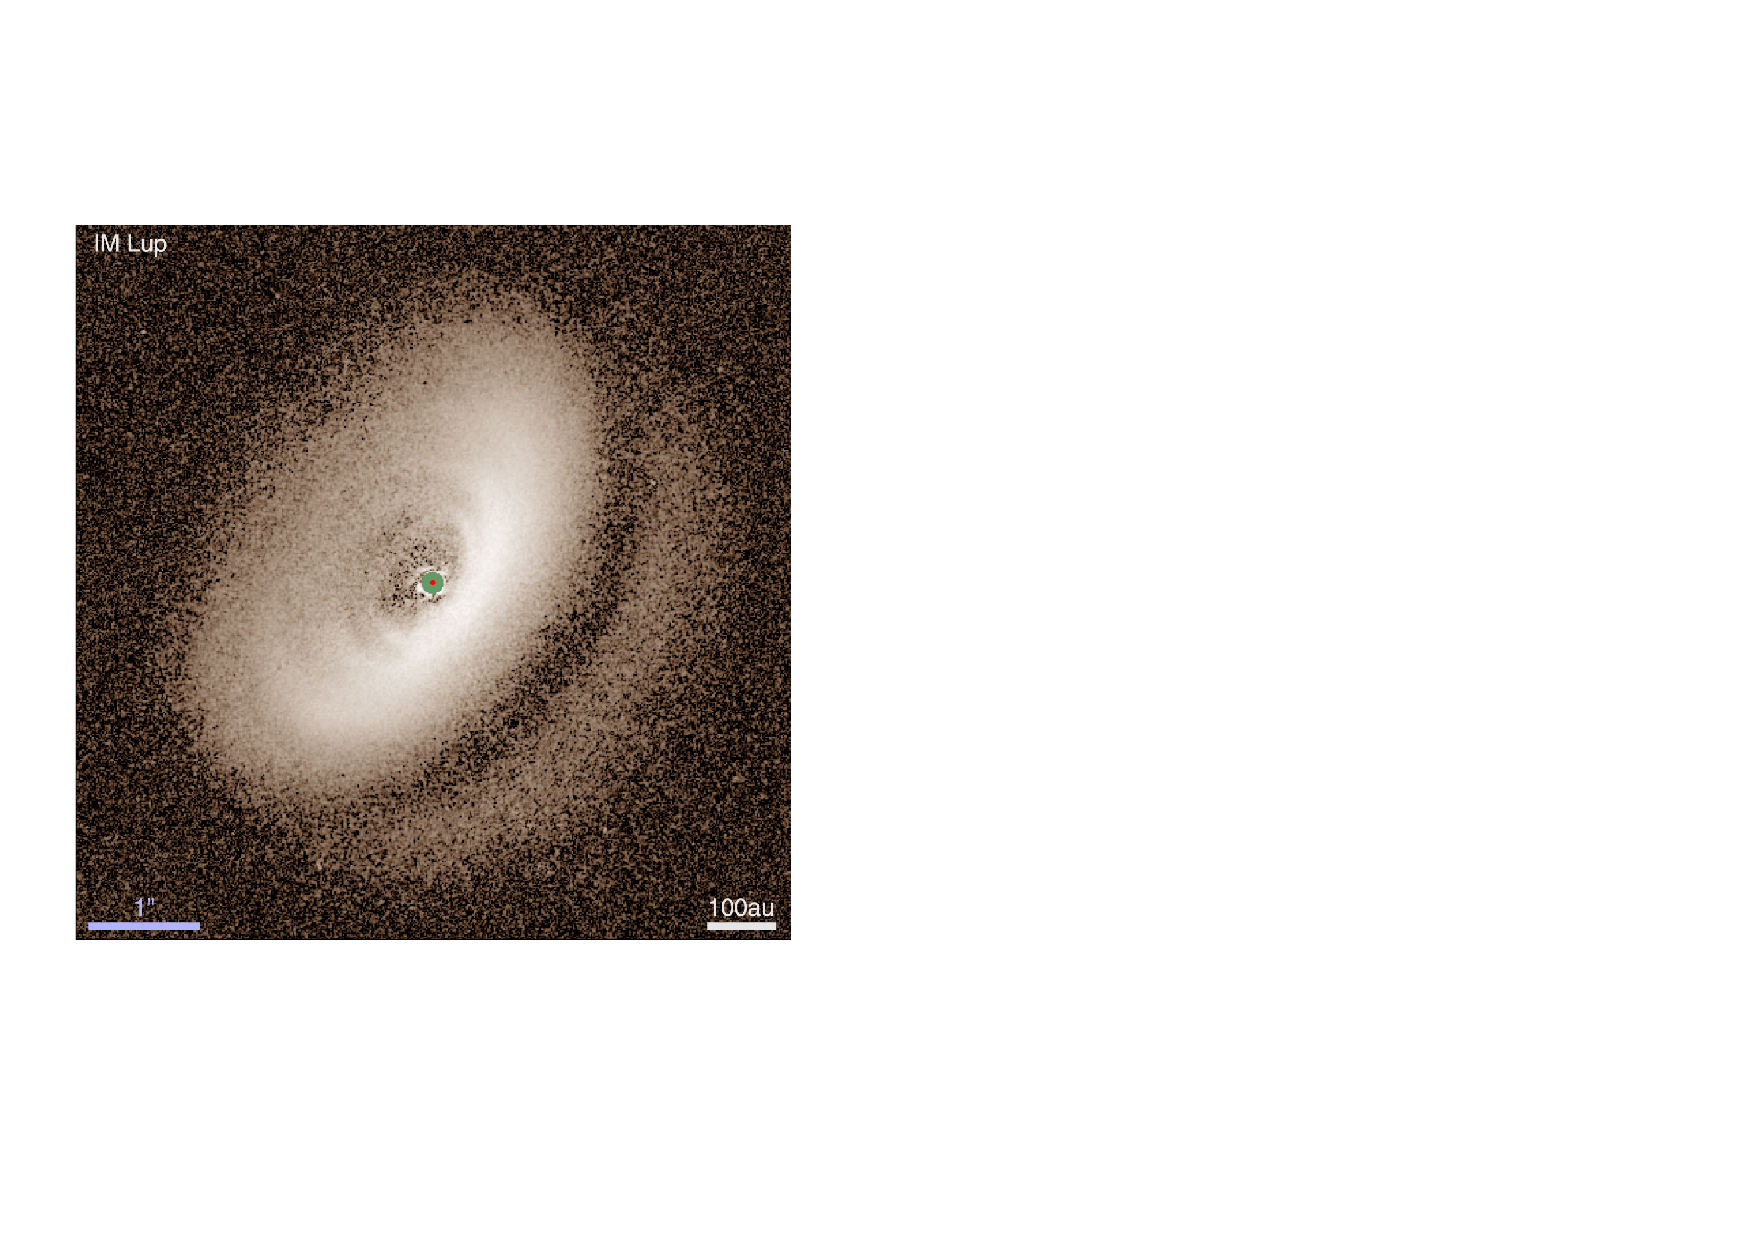
\includegraphics[width = 0.5\textwidth]{figures/IM_Lup_scattered.pdf}
    \caption{H-band image showing the light scattered off the top and bottom surfaces of the disk around the T-Tauri star IM~Lupi, taken with the extreme adaptive optics SPHERE instrument at the Very Large Telescope \citep{avenhaus2018}.
    The data has been rescaled with a logarithmic stretch to improve contrast.
    The green dot in the centre of the image corresponds to a region where no data was taken due to the coronagraph, the red dot is the star position.
    1 arcsecond and 100 au scales are in the bottom left and right of the image respectively.
    The disk clearly exhibits the flared structure expected for centrally illuminated disks.}
    \label{fig:im_lup}
\end{figure}

\section{Viscous Evolution}

Combining the mass and angular momentum conservation Equations \eqref{eq:1d_cont} and \eqref{eq:1d_angmom}, and substituting the Keplerian forms for $\Omega$ and $h$ in Equations \eqref{eq:point_pot} and \eqref{eq:ang_mom}, we find
\begin{align}
    \partial_t \Sigma &= \frac{3}{r} \partial_r \left[ \sqrt{r} \partial_r \left( \nu \sqrt{r} \Sigma  \right)  \right] \label{eq:1d_evol},
\end{align}
which gives the evolution in the surface density for a thin, Keplerian disk.
The Equation~\eqref{eq:1d_evol} has the form of the one-dimensional heat or diffusion equation, and its diffusive properties are evident in the \textit{ring spreading} solution derived by \citet{lynden-bell1974} in the case of constant $\nu$.
The initial condition for this solution is the Dirac delta centred at $r/r_0 = 1$, representing a thin ring of material orbiting at some radius.
The solution shown in Figure~\ref{fig:ring_spreading}, and we see that the diffusion results in the movement of a lot of mass to small radii, while small amounts of mass carry angular momentum away to very large radii.

\begin{figure}
    \centering
    \includegraphics[width = 0.8\textwidth]{figures/armitage_ringspread.png}
    \caption{The evolution of a ring of gas centred initially at $r=r_0$ according to Equation~\eqref{eq:1d_evol}, as derived by \citet{lynden-bell1974}. Each curve is plotted from $\tau=0.008$ to $\tau=0.512$ with interval 0.084, where $\tau$ is dimensionless time \citep[figure from lecture notes by][]{armitage2022}. The diffusive nature of the evolution is clearly evident, with the overdense ring spreading out over time.}
    \label{fig:ring_spreading}
\end{figure}

The analysis here and in Section~\ref{sec:fluid_eqns} relies on viscous disk theory as previously stated.
In this, we consider that although angular momentum may be physically transferred by mechanisms such as the magnerotational instability \citep{sano2000}, self-gravity \citep{kratter2016}, turbulent eddies \citep{klahr2003}, or others, we assume that all of the physics can be captured by the kinematic viscosity $\nu$.
Modelling disk evolution accurately therefore relies on determining the value of $\nu$.
\citet{shakura1973} argued that it is physically consistent to parametrise the viscosity in terms of some constant $\alpha \lesssim 1$ as\footnote{Strictly there is also a factor of $2/3$ on the right-hand side but this is typically ignored in the literature and absorbed into the value of $\alpha$.}
\begin{align}
    \nu = \alpha c H.
\end{align}
This is known as the $\alpha$\textit{-prescription}. If $\nu \propto r^\beta$ for some constant real number $\beta$, then \eqref{eq:1d_evol} has solution \citep{lynden-bell1974}
\begin{align}
    \Sigma(r) = (2 - \beta) \frac{M_d}{2 \pi r_c^2} \left( \frac{r}{r_c} \right)^{-\beta} \exp{\left[ - \left(\frac{r}{r_c}\right)^{2-\beta} \right]}, \label{eq:exp_taper_dens}
\end{align}
which is a so-called \textit{exponentially tapered} power law in $\Sigma$.
That is, the density roughly obeys a negative power law with index $-\beta$ at radii less than the critical radius $r_c$, while dropping off exponentially at radii greater than $r_c$.
Using the $\alpha$-prescription and the definition of $\gamma$ given in Equation~\eqref{eq:flared_hr} gives $\beta=2\gamma+\frac{1}{2}$.
More commonly this is parameterised in terms of the effective temperature profile or the sound speed profile $T \propto c^2 \propto r^{-2q}$ for some constant real number $q$, yielding $\beta = \frac{3}{2} - 2q$ \citep{hartmann1998}.
If we take $q=1/4$ as in Section~\ref{sec:disk_flaring}, then $\beta=1$ \citep{chiang1997}.

The exponentially tapered power law picture for the surface density profile \eqref{eq:exp_taper_dens}, combined with the vertically Gaussian density structure \eqref{eq:vertical_rho}, provide the typical parameterisation used to fit the density structure of observed disks \citep{andrews2011,zhang2021}.
The high-resolution MAPS survey found remarkably consistent best fitting parameters of $\beta=1$ and $\gamma=0.2$, with variation of only $\simeq20$\% and $\simeq10$\% respectively across the 5 disks in the sample.

\section{Observed Properties}

\subsection{Components}

Figure~\ref{fig:struct_cartoon} presents a cartoon overview of the modern understanding of the structural components of protoplanetary disks \citep{andrews2020}.
The disk is comprised of both gas and dust, where dust is taken to mean any solid material.
The gas component is pressure supported and so exhibits the expected flared structure discussed in Section~\ref{sec:disk_flaring}.
The dust grains however do not feel any pressure and their behaviour depends on their size.
Small dust grains, those on the order of a few microns or less, couple strongly to the gas and thus trace the gas structure.
Larger grains experience drag forces and thus settle to the disk mid-plane \citep{weidenschilling1977}.
These different components are probed via different observational tracers.
The distribution of small dust grains may be examined through scattered light, while the larger grains can be traced with millimetre thermal continuum observations \citep{almapartnership2015,andrews2016,ansdell2016}. 
The gas component on the other hand may be studied through spectral emission lines of different molecules.
These kinds of observations can be used to constrain the gas gas distribution \citep{vandermarel2015,ansdell2016,zhang2021}, kinematics \citep{perez2015,pinte2018a,teague2018,pinte2019,yu2021,calcino2022} and temperature \citep{pinte2018,calahan2021}.

\begin{figure}
    \centering
    \includegraphics[width = 0.99\textwidth]{figures/cartoon_overview.pdf}
    \caption{A cross section schematic of a typical protoplanetary disk. The location of gas is shown in grey while dust grains and larger solids are shown in purple. Labels on the left outline key observational tracers of disk structure while the labels on the right identify those features. The figure is intended as a rough outline and is not to scale \citep[see review by][]{andrews2020}. The pressure support of the gas results in a thick disk extended in the vertical direction, while the large dust grains settle to a thin layer in the mid-plane.}
    \label{fig:struct_cartoon}
\end{figure}

\subsection{Size}

The size of a disk is typically defined as the radius within which 90\% of the total luminosity is contained.
This is in general a function of the observational tracer and so for example $R_\mathrm{mm}$ may be different to $R_\mathrm{CO}$, where the subscripts signify millimetre continuum and molecular carbon monoxide (CO) line emission respectively. 
Furthermore, each of these sizes may be used as a proxy for the size of a certain component of the disk based on what the component of the disk probes.
Thus $R_\mathrm{mm}$ is essentially the size of the dust disk comprised of millimetre sized grains and larger, while $R_\mathrm{CO}$ gives the size of the gas disk.
In general the size of the dust disk is smaller than the gas disk for the same system, as demonstrated in Figure~\ref{fig:maps_disks}.
Medium resolution population studies that resolved almost 200 disks to scales of $25-50$ au suggest that the typical dust disk size is in the $\simeq 10 - 250$ au \citep{tripathi2017,andrews2018a,hendler2020}.
This range is supported by surveys of many fewer disks, around 30, taken at the much higher resolution of $\sim5$ au \citep{long2018,huang2018b}.
The gas disks are typically larger with radii of $100 - 500$ au, with a few extending out even farther \citep{ansdell2018,zhang2021}.

\begin{figure}
    \centering
    \includegraphics[width = 0.95\textwidth]{figures/Figure-DISKS-Website.png}
    \caption{Top row: $^{12}$CO $2-1$ Line emission integrated intensity images taken of the five protoplanetary disks as part of MAPS \citep{oberg2021}.
    The bottom row shows continuum millimetre observations of the same disks, zoomed in on the box shown on each figure in the top row \citep{andrews2018,huang2020,oberg2021}. 
    We see that in each case the spatial extent of the dust disk probed in mm is much less than that for the gas disk probed with $^{12}$CO.
    Figure retrieved from \url{https://www.alma-maps.info/disks.html}.}
    \label{fig:maps_disks}
\end{figure}

\subsection{Mass}

Observational disk mass measurements are something of a problem child.
We split the total disk mass $M_\mathrm{d}$ into two components, the gas mass $M_\mathrm{g}$  and the dust or solids mass $M_\mathrm{s}$ where $M_\mathrm{d} = M_\mathrm{g} + M_\mathrm{s}$.
Measurements of $M_\mathrm{s}$ rely on assumptions of the optical properties of dust grains and so are intrinsically uncertain.
$M_\mathrm{g}$ measurements are even worse off.
Molecular hydrogen is too faint in disks to be of use, no instruments operating or planned can observe the hydrogen deuteride $1-0$ transition that may be of use, and most other molecules are not very abundant.
CO is the next most abundant molecule after $H_2$ and is readily detectable at wavelengths available to ALMA.
Measurements of $M_\mathrm{g}$ via CO are unfortunately complicated by uncertainty in the C/H ratio in disks \citep[see the review by][for in-depth discussion of difficulties with disk mass measurements]{miotello2022}.

These measurements are crucial to understanding planet formation as they constrain the possible bodies that may be created from a disk as it continues to evolve.
The \textit{Minimum Mass Solar Nebula} (MMSN) is the hypothesised disk that the solar system formed from, with just enough mass to create each of the planets \citep{hayashi1981}.
Modern measurements place the MMSN at $M_\mathrm{s} \gtrsim 40 \, \mathrm{M_\oplus}$ (where $\mathrm{M_\oplus}$ is an Earth mass), $M_\mathrm{g} \gtrsim 3000 \, \mathrm{M_\oplus}$, where $\mathrm{M_\oplus}$ is an Earth mass \citep[see review by][]{andrews2020}.
If planets are formed from protoplanetary disks then the mass of said disks should be comparable to, or larger than, the MMSN.
Figure~\ref{fig:disk_masses} shows the distribution of dust mass measurements for disks in the regions of Ophiuchus, Lupus, Upper Scorpius, Chamaeleon I, $\sigma$ Ori, IC 348 and Taurus \citep[and references therin]{cieza2019}, compared with the MMSN.
Even in the youngest regions of the sample, fewer than $20\%$ of the disks contain a dust mass greater than the MMSN value of $M_\mathrm{s}\gtrsim 40 \, \mathrm{M_\oplus}$.
This result does not seem to be compatible with the known population of exoplanets, a conundrum known as the \textit{missing mass problem} \citep[e.g.][]{najita2014}.

One possible resolution to the missing mass problem is that protoplanetary disks are planet-hosting disks rather than planet-forming disks.
In this scenario planet formation occurs during the protostellar stage while the star is still embedded in a envelope, since massive disks are more common \citep{greaves2010}.
This scenario is supported by the growing body of evidence that protoplanetary disks contain planets when the system is as young as 1-2 Myr \citep{almapartnership2015,zhang2018,verrios2022}.
On the other hand planet formation may be incredibly efficient during the very early protoplanetary stage \citep{najita2014,manara2018,Tychoniec2020}.
A final possibility is that derived dust disk masses suffer from systematic underestimation. 
\citet{zhu2019} argued that if disks are not optically thin, as assumed in calculations of disk mass from continuum observations, then the true dust mass may be a factor of 2 or more larger.
Whatever the case may be, it is likely that detecting young planets and constraining their masses through kinematic observations will be a key part of determining which scenario is correct.

\begin{figure}
    \centering
    \includegraphics[width = 0.7\textwidth]{figures/disk_mass.pdf}
    \caption{Cumulative mass distributions for disks found in various nearby young stellar regions. The shaded regions represent the $1\sigma$ confidence intervals \citep{vanterwisga2019}. Plotted in red is the dust mass of the MMSN \citep{weidenschilling1977b}. According to this analysis, very few of the disks in the sample have enough mass to create the planets of the solar system.}
    \label{fig:disk_masses}
\end{figure}

    \chapter{The Planet-Disk Interaction}
    \section{Spiral Density Waves}

\section{The Linear Disk Response}

\subsection{WKBJ Dispersion Relation}

\subsection{Lindblad Resonances}

\subsection{The Planet Wake}

\subsection{Additional Spiral Arms}

\section{Non-Linear Wake Evolution}

\subsection{Angular Momentum Flux}

\section{Gap Formation}

    \chapter{Semi-Analytic Models of Planet Wakes} \label{ch:wake_models}
    \setlength{\headheight}{13.59999pt}

This chapter is concerned with the method we have used to create semi-analytic models of planet wakes that encompass both the linear and non-linear disk response due to a perturbing planet as described in the previous chapter. 
Section \ref{sec:JOSS} introduces our Python package \textsc{wakeflow}, while sections \ref{sec:diskstruct}-\ref{sec:wakeprop} outline the theory and numerical methods it uses.

\section{Wakeflow: A Python Package For Semi-Analytic Models of Planet Wakes} \label{sec:JOSS}

This section has been published in the Journal of Open Source Science \fct and is publicly available here \fct

\subsubsection{Summary}

\textsc{wakeflow} is a Python package for generating semi-analytic models of the perturbations induced by planets embedded in gaseous circumstellar disks. 
These perturbationstake the form of a spiral shock wave \citep{ogilvie2002}, and are often called a "planet wake" in analogy with that produced by a boat in a lake.

\subsubsection{Statement of Need}

Detecting newly formed planets embedded in their disk is a challenging problem in the field of planet formation. 
A major area of progress in recent years isthe detection of planets by the gravitationally induced disturbance in theirhost disks. 
This disturbance, caused by the planet wake, manifests as a deviation in velocity from the bulk flow which may be measured through the Doppler shift of molecular lines \citep[eg.][]{perez2015, pinte2018a}. 
Such kinematic observations have been accurately reproduced through 3D fluid simulations of the planet-disk interaction, allowing for the inference of planet and disk properties \citep{pinte2018a, pinte2019}. 
However, these studies are computationally expensive.

\textsc{wakeflow} eases this computational cost by applying the theory of planet wake generation and propagation \citep{goldreich1979,goodman2001,rafikov2002a,bollati2021}to create semi-analytic models of planet wakes. 
\textsc{wakeflow} models are readily created in less than a minute on a modern laptop, as opposed to the hours of supercomputer time needed for 3D hydrodynamical simulations. 
The relatively low computational cost of \textsc{wakeflow}means that researchers can get an idea of whether planet-disk interactionscan explain their observations, and the disk and planet parameters needed, beforespending computer time on more detailed simulations.

\textsc{wakeflow} can interface with the radiative transfer code  \textsc{mcfost} \citep{pinte2006,pinte2009} in order to create synthetic observations of the semi-analytic models for direct comparison with observed continuum or line emission.

\textsc{wakeflow} is partially adapted from a previous Python code also written by us called \textsc{analytical\_kinks} [@Analytical\_Kinks]. 
\textsc{wakeflow} is intended to be a more complete, versatile and easy to use version of that code, and it obeys standard Python packaging conventions.
In addition, \textsc{wakeflow} can directly interface with \textsc{mcfost} while \textsc{analytical\_kinks} cannot.
At the time of writing, no other open source software packages exist to generate the perturbations induced by an embedded planet in a circumstellar disk using the semi-analytic theory of planet wakes.

Existing scientific publications focusing on detecting the kinematic signatures of planets that have used \textsc{wakeflow} or its predecessor \textsc{analytical\_kinks} include \citet{bollati2021}, \citet{calcino2022}, \citet{teague2022}, \citeauthor{garginreview} (in review) and \citeauthor{fasanoinprep.} (in prep.).

\subsubsection{Acknowledgements}

\textsc{wakeflow} relies on the following scientific Python packages: \textsc{NumPy} \citep{harris2020}, \textsc{matplotlib} \citep{hunter2007}, \textsc{SciPy} \citep{virtanen2020} and \textsc{Astropy} \citep{astropycollaboration2022}.

\section{Semi-Analytic Solution Algorithm}

As stated in the previous section, \textsc{wakeflow}

Outline the wakeflow algorithm for generating a model:
\begin{enumerate}
    \item Generate grid geometry. Interface with \textsc{mcfost if desired}.
    \item Calculate the unperturbed disk.
    \item Read in linear perturbations, scale, interpolate onto global grid geometry interpreting $y$ as an arc length in $\phi$. Mapped onto an annulus. Annulus is an update, more honestly displays results from shearing sheet approximation, minimises discontinuity in solution. Also, it is perfectly acceptable to extend the box vertically further since it is the position of the Lindblad resonances that matter ultimately for the linear regime not the planet itself (sort of).
    \item Extract initial conditions using \textbf{exact} transformations instead of approximate ones in \citet{bollati2021} to minimise discontinuity in solution.
    \item Solve Burger's equation until $t_{\rm f}=300$ using vectorised Godunov solver and adaptive time stepping.
    \item Get $\chi(r,\phi)$. Transformations are vectorised and the whole solution is interpolated in one go. Asymptotic regime and planet annulus are masked.
    \item Perturbations are calculated from $\chi$ using updated velocity mapping
\end{enumerate}

\section{Theoretical and Numerical Considerations} 

\note{Add something about how we are basically going into more detail for the steps in the algorithm and explaining the specific applications of or improvements to the stuff that been done before.}

\subsection{Unperturbed Disk Structure} \label{sec:diskstruct}

Here we outline the unperturbed disk model used in \textsc{wakeflow} onto which the perturbations are added.

\subsubsection{Temperature}

We assume that the sound speed $c$ obeys a simple radial power law 
\begin{align}
    c \propto r^{-q},
\end{align}
where $q$ is some real number. Thus the disk temperature scales as 
\begin{align}
    T \propto c^2 \propto r^{-2q}.
\end{align}
The constant of proportionality for these relations in determined by the user specified value of the disk aspect ratio $H/r$ at $r=r_{\rm ref}$

\subsubsection{Density}

We use a density structure derived by assuming that the disk is in vertical hydrostatic equilibrium \citep{pringle1981}, but unlike in \ref{eq:vertical_rho} we will not assume that $z\ll r$.
The density $\rho$ is given by 
\begin{align}
    \rho(r,z) \propto \left( \frac{r}{r_{\rm ref}} \right)^{-p} \exp{\left( \frac{G M_\star}{c^2} \left[ \frac{1}{\sqrt{r^2 + z^2}} - \frac{1}{r} \right] \right)},
\end{align}
where $p$ is some real number. 
The constant of proportionality is set directly by the user, or calculated by \textsc{mcfost} based on the total gas mass.

Very commonly the density profile is parameterised in terms of the surface density $\Sigma$, not the actual density $\rho$ as above.
If the surface density is parameterised as $\Sigma \propto r^{-\delta}$ where $\delta$ is some real number, then equation \ref{eq:surf_dens_to_dens} gives the approximate relation 
\begin{align}
    p \simeq \frac{3}{2} - q + \delta,
\end{align}
which can be used to convert between density parameterisations.
This conversion is only approximate in our context, since is does assume that $z \ll r$ and our density profile does not.
However this turns out not to matter since $\delta$ will only show up in the $t(r)$ mapping which we will assume is the same for all $z$.

\subsubsection{Velocities}

The radial and vertical motions in the unperturbed disk are set to zero. 
The rotation is derived assuming radial force balance \citep[eg.][]{nelson2013} and is given by 
\begin{align}
    \Omega(r,z) = \Omega_{\rm K} \left[ - \left(p + 2q\right) \left( \frac{H}{r} \right)^2 + \left( 1-2q \right) + \frac{2qr}{\sqrt{r^2 + z^2}}\right]^{1/2},
\end{align}
where $\Omega_{\rm K}$ is as defined in equation \ref{eq:point_pot}.

\subsection{Transformations}

\note{Something about we give the transformations used in mapping from $(r,\phi)$ to $(t,\eta)$ space. We use parameterisations of sound speed and surface density}
\begin{align}
    c(r) = c_{\rm p} \left(\frac{r}{r_{\rm p}}\right)^{-q}; \quad \Sigma(r) = \Sigma_{\rm p} \left(\frac{r}{r_{\rm p}}\right)^{-\delta},
\end{align}
where $c_{\rm p}$ and $\Sigma_{\rm p}$ are the sound speed and surface density at $r_{\rm p}$.
Assuming also that $\Omega=\Omega_{\rm K}$, then equation \ref{eq:phi_wake} becomes \citep{rafikov2002a}
\begin{align}
    \phi_{\rm wake}(r) = \phi_{\rm p} + {\rm sgn} \left( r - r_{\rm p} \right) \frac{r_{\rm p}}{H_{\rm p}} \left[ \frac{2}{2q-1} \left(\frac{r}{r_{\rm p}}\right)^{q-\frac{1}{2}} - \frac{1}{q+1} \left(\frac{r}{r_{\rm p}}\right)^{q+1} - \frac{3}{\left(2q-1\right)\left(q+1\right)} \right].
\end{align}
Additionally, the Keplerian rotation implies $|2A| = 3\Omega/2 = 3c/2H$ and so the Mach-1 length becomes
\begin{align}
    l_{\rm p} = \frac{2H}{3},
\end{align}
and so the $\eta$ transformation \ref{eq:eta} reduces to 
\begin{align}
    \eta(r, \phi) = \frac{3 r_{\rm p}}{2 H_{\rm p}} \left[ \phi - \phi_{\rm wake} \right].
\end{align}
Additionally the $t$ transformation becomes \citep{rafikov2002a}
\begin{align}
    t(r) = \frac{3}{2^{5/4}} \left( \frac{r_{\rm p}}{H_{\rm p}} \right)^{\frac{5}{2}} \left| \int_1^{r/r_{\rm p}} |s^\frac{3}{2} - 1|^\frac{3}{2} s^{\frac{5q+\delta}{2}-\frac{11}{4}}\, ds \right|, \label{eq:t_power}
\end{align}
where explicitly the $g$ function is given by \citep{bollati2021}
\begin{align}
    g(r) = 2^{1/4} \left( \frac{r_{\rm p}}{H_{\rm p}} \right)^{\frac{1}{2}} \frac{\left( \frac{r}{r_{\rm p}} \right)^{\frac{5}{4} - \frac{\delta + 3q}{2}}}{\left| 1 - \left(\frac{r}{r_{\rm p}}\right)^\frac{3}{2} \right|^\frac{1}{2}}
\end{align}
This gives us all the tools we need to map from $(r,\phi)$ space to $(t,\eta)$ space in a Keplerian power law disk.
These are the forms of the transformations used by \textsc{wakeflow}.
We are therefore implicitly assuming that the unperturbed rotation profile is well approximated as Keplerian in the midplane, which is reasonable since the correction is of order $\left(H/r\right)^2$.

Unlike in \citet{goodman2001,rafikov2002a,bollati2021} we do not use approximate forms of the transformations that hold nearby the planet in the shearing sheet approximation to extract the initial condition for the Burger's evolution.
We found that the approximate transformation for $\eta$ \citep[equations 35 in][]{rafikov2002a} shifted the wake profile in $\eta$ by a few percent, leading to a discontinuity in the solution at the interface between the linear and non-linear regimes.
The approximate $t$ transformation has a similar effect although it is much smaller.
For this reason we always use the exact transformations as listed above.

After Burger's equation is solved numerically, the solution must be mapped from $\chi(t,\eta)$ to $\chi(r,\phi)$.
Since $t(r)$ is not invertible, we instead find the $(t,\eta)$ coordinates of every point on the solution grid $(r,\phi)$ and interpolate from the Burger's solution in $t,\eta$ space.
We therefore must evaluate the $t(r)$ and $\eta(r,\phi)$ transformations $N$ times, where $N$ is the number of points in the grid.
The $\eta$ transformation is easily vectorised since it is a simply algebraic expression, however the $t(r)$ transformation \ref{eq:t_power} involves an integral which naively must be evaluated $N$ times.
This approach is very inefficient, since the integral in the transformation does not actually depend on $r$, merely the end point does.
Re-evaluating the integral each time therefore often involves integrating over the same interval very many times.
In \textsc{wakeflow} we instead convert mapping $r\rightarrow t$ into an initial value problem (IVP).
Since the integrands of equation \ref{eq:t} is independent of r, we can convert equation \ref{eq:t} into an ordinary differential equation with an appropriate initial condition
\begin{align}
    \frac{dt(s)}{ds} = \frac{r_{\rm p}}{l_{\rm p}} \left[ \frac{\Omega(s) - \Omega_{\rm p}}{c_0(s) g(s)} \right]; \quad \, t(r_{\rm p}) = 0.
\end{align}
where obtaining $t(r)$ from the solution $t(s)$ is simply a matter of taking $s=r$.
Applying this analysis to the $t$ transformation for a power law disk \ref{eq:t_power} we obtain 
\begin{align}
    \frac{dt(s)}{ds} = \frac{3}{2^{5/4}} \left( \frac{r_{\rm p}}{H_{\rm p}} \right)^{\frac{5}{2}} \left| |s^\frac{3}{2} - 1|^\frac{3}{2} s^{\frac{5q+\delta}{2}-\frac{11}{4}} \right|; \quad t(1)=0, \label{eq:t_power_IVP}
\end{align}
and $t(r)$ is obtained from the solution taking $s=r/r_{\rm p}$.
\textsc{wakeflow} calculates the $t$ coordinates of the grid points by solving the IVP \ref{eq:t_power_IVP} using the \textsc{SciPy} function \textit{integrate.odeint} \citep{virtanen2020}.

\subsection{Velocity Perturbations} \label{sec:velocity_perts}

As we saw in section \ref{sec:nonlinear_evolution} the conservation of the Riemann invariant $R_+$ gives for the radial velocity perturbation
\begin{align}
    u = 2\frac{c_0-c}{\gamma - 1}=-2\frac{c_0}{\gamma + 1} \psi, \label{eq:u_rafikov}
\end{align}
where we define $\psi$ as
\begin{align}
    \psi = \frac{\gamma+1}{\gamma-1} \frac{c - c_0}{c_0},
\end{align}
which is the sound speed perturbation with a constant scale factor. Following \citet{rafikov2002a}, we then derive an expression for $\psi$ in terms of the density perturbation $\chi$ by assuming that the gas obeys a locally polytropic equation of state given by 
\begin{align}
    P = P_0(r) \left[ \frac{\Sigma}{\Sigma_0(r)} \right]^\gamma. \label{eq:poly_EOS}
\end{align}
The sound speed is then
\begin{align}
    c^2 = \frac{\partial P}{\partial \Sigma} = c_0^2(r) \left[ \frac{\Sigma}{\Sigma_0(r)} \right]^{\gamma-1}.
\end{align}
\citet{rafikov2002a} then finds a relation between the density and sound speed perturbations, accurate to second order in $\psi$, found by expanding the above expression. 
This yields
\begin{align}
    \frac{\Sigma - \Sigma_0}{\Sigma_0} = \frac{2}{\gamma + 1}\psi + \frac{3 - \gamma}{\left( \gamma + 1  \right)^2} \psi^2 + \mathcal{O}(\psi^3). \label{eq:psi_exp}
\end{align}
Taking this expression to first order only, we write $u$ in terms of the density perturbation, and then in terms of $\chi$ by substituting Equation \feqr. 
\begin{align}
    u = - c_0 \frac{\Sigma - \Sigma_0}{\Sigma_0} = -2 \frac{c_0}{\gamma + 1} \frac{\chi}{g(r)}. \label{eq:ap_rad_vel}
\end{align}
Similarly, \citet{rafikov2002a} finds the azimuthal velocity as
\begin{align}
    v \approx -2 \frac{c_0^2}{\Delta\Omega r} \frac{1}{\gamma + 1} \psi, \label{eq:v_rafikov}
\end{align}
giving to first order in $\psi$
\begin{align}
    v \approx - \frac{c_0^2}{\Delta \Omega r} \frac{\Sigma - \Sigma_0}{\Sigma_0} = - \frac{2}{\gamma + 1} \frac{c_0^2}{\Delta \Omega r} \frac{\chi}{g(r)}. \label{eq:ap_az_vel}
\end{align}
Equations \ref{eq:ap_rad_vel} and \ref{eq:ap_az_vel} are the expressions used in \citet{bollati2021} to calculate the velocity perturbations in the non-linear regime. 
Since these are only accurate to first order in $\psi$, the assumption is made that $\psi \ll 1$; indeed \citet{bollati2021} notes that terms proportional to $\psi^2$ are discarded in the derivation of the Burgers evolution \feqr, and thus also in the calculation of $\chi$ from which $u$ and $v$ are calculated. 
However it is not clear that neglecting the most non-linear terms to calculate the density perturbation $\chi$ necissitates the truncation of the equation of state in the same way. 
Since we are in particular interested in the velocity perturbations, and in planet masses comparable to the thermal mass, we should check if the assumption that $\psi \ll 1$ holds.

We can derive an \textit{exact} expression for $\psi$ in terms of the density perturbation simply by rearranging Equation \ref{eq:poly_EOS}. We find
\begin{align}
    \psi = \frac{\gamma + 1}{\gamma - 1} \left[ \left( \frac{\Sigma-\Sigma_0}{\Sigma_0} +1  \right)^{(\psi-1)/2}  -1 \right],
\end{align}
which can be written equivalently in terms of $\chi$ using Equation \feqr giving
\begin{align}
    \psi = \frac{\gamma + 1}{\gamma - 1} \left[ \left( \frac{2}{\gamma + 1} \frac{\chi}{g(r)} +1  \right)^{(\psi-1)/2} -1 \right]. \label{eq:psi_exact}
\end{align}
We will use Equation \ref{eq:psi_exact} to check the aforementioned assumption that $\psi \ll 1$ in the non-linear regime solution. 
We construct three \textsc{wakeflow} models using dimensionless units, with embedded planet masses of $0.5, 1.0$ and $2.0 \, M_{\rm{th}}$ respectively, all placed in orbit around a $1 \, M_{\rm{\odot}}$ star at an orbital radius of $r=1$. 
For all models, we choose $p=2.25$ and $q=0.25$ such that $\Sigma \propto r^{-1}$, and an aspect ratio $H/r=0.1$ at $r=1$. 
Figure \ref{fig:psi_comparison} shows the values of $\psi$ for each of these models, and demonstrates that even for the lowest planet mass model the value of $\psi$ nearby the planet is as large as $\sim \hspace{-0.23em} 0.6$ and so the second order terms will clearly be important even in this case. 
For masses $\ge \hspace{-0.23em} M_\mathrm{th}$ the problem is even worse, as there are regions where $\psi \gtrsim 1$ causing the expansion given in Equation \ref{eq:psi_exp} to diverge.

\begin{figure}
    \centering
    \includegraphics[width = 0.98\textwidth]{figures/psi 2.pdf}
    \caption{Comparison of the values of $\psi$ calculated from Equation \ref{eq:psi_exact} for three \textsc{wakeflow} models with planet masses of $0.5, 1.0$ and $2.0 \, M_{\rm{th}}$ respectively. Clearly one cannot assume that $\psi \ll 1$ even for the lowest mass model, especially nearby the planet. For the two larger masses, there are even regions where $\psi > 1$.}
    \label{fig:psi_comparison}
\end{figure}

To improve upon the velocity calculations used in \citet{bollati2021}, here we derive expressions for both $u$ and $v$ as functions of $\chi$ without truncating the equation of state to first order in $\psi$. This is as simple as substituting Equation \ref{eq:psi_exact} into Equations \ref{eq:u_rafikov} and \ref{eq:v_rafikov}, yielding
\begin{align}
    u(\chi) &= -2 \frac{c_0}{\gamma - 1} \left[ \left( \frac{2}{\gamma + 1} \frac{\chi}{g(r)} +1  \right)^{(\psi-1)/2} -1 \right] \\
    v(\chi) &\approx \frac{c_0}{\Delta\Omega r} u (\chi).
\end{align}




which are the expressions used to calculate the velocity perturbations in the non-linear regime in \textsc{wakeflow}. 

\begin{figure}
    \centering
    \includegraphics[width = 0.7\textwidth]{figures/0_5_mth.pdf}
    \caption{}
    \label{fig:0_5mth}
\end{figure}

\begin{figure}
    \centering
    \includegraphics[width = 0.7\textwidth]{figures/1_0_mth.pdf}
    \caption{}
    \label{fig:1_0mth}
\end{figure}

\begin{figure}
    \centering
    \includegraphics[width = 0.7\textwidth]{figures/2_0_mth.pdf}
    \caption{}
    \label{fig:2_0mth}
\end{figure}



\section{Synthetic Kinematic Observations}

\subsection{Predictions from 2D Models}

\subsection{3D Models}

\subsection{Radiation Transfer}

    \chapter{Mapping the Planet Wake in HD~163296 with Kinematics} \label{ch:wake_mapping}
    
\section{Introduction}

\section{Methods}

\subsection{Observations}

\subsection{Hydrodynamical Simulations and Radiation Transfer}

\subsection{Spiral Wake Mapping}

\section{Results}

\section{Discussion}

\subsection{Density Waves or Buoyancy Spirals?}

\subsection{Estimating the Planet Mass}

\subsection{Model Limitations}

\section{The Planet Wake in IM Lupi} \label{sec:IMLupiwake}

    \chapter{Quantitative Measurements of the Wake}
    The final section of the thesis is concerned with trying to constrain the mass of protoplanets embedded in disks by quantitatively extracting the planet wake from kinematic observations.
We will build on the work presented in \citet{calcino2022}, where we showed that one can trace the shape of the planet wake, and amplitude of velocity kinks, through the peak velocity map.
In Section~\ref{sec:v0_fitting} we attempt to create a planet mass fitting procedure using synthetic peak velocity maps generated by projecting \textsc{wakeflow} models to the emitting surface of the disk.
Additionally, in Section~\ref{sec:mirror_residuals}, we present a method for locating the wake such as that in \citet{calcino2022}, but that does not rely on identifying patterns by eye.
%Finally in Section~\ref{sec:isovelocity_transform}, we demonstrate a potential method for extracting the wake information from observations that is model-independent.

\section{Peak velocity fitting} \label{sec:v0_fitting}

As shown in \citet{calcino2022}, the planet wake manifests in the peak velocity ($v_0$) map generated from molecular line emission observations as spatially correlated deviations from the expected smooth iso-velocity contour.
We additionally created synthetic $v_0$ maps by projecting semi-analytic models of the planet wake plus background rotation (Equation~\ref{eq:rot_eq_full}) to a the emitting layer of the disk, and then calculating the line-of-sight velocities in the disk.
Here, we will take the same approach to generating $v_0$ maps, but we will fit them onto the observed peak velocities.
The advantage of fitting in this way instead of first subtracting a best-fitting model for the background rotation and fitting to the residuals is two-fold.
First, creating residuals in this way is known to easily confuse the sign of the perturbations due to the high sensitivity to the background model (see the Appendix of \citealt{calcino2022}).
Secondly, fitting simultaneously for the background instead of assuming it allows for the determination of the covariances in the uncertainties between the background and planet perturbation models.
The best-fitting parameters for the planet mass and location will therefore not be conditioned on some background model, and we will be able to see any potential degeneracies between the parameters of each model.

\subsection{Models}

To generate our models, we first calculate the height of the emitting layer in the disk using the parameterisation \citep{pinte2018}
\begin{align}
    z(r) = z_0 \left( \frac{r}{r_{\rm ref}} \right)^\phi \exp \left( -\left[ \frac{r}{r_\mathrm{taper}} \right]^{\psi} \right), \label{eq:height}
\end{align}
which gives a flared structure with an exponential taper. $z_0$, $\phi$, $r_{\rm taper}$ and $\phi$ are then all model parameters that determine the height of the emitting layer. 
$r_{\rm ref}$ simply determines the radius at which the reference height $z_0$ and other parameters are defined, and we just set it to 100 au.
While this is a lot of freedom, the idea is to eventually use other methods of determining the height in this form such as the code \textsc{dynamite}\footnote{\url{https://github.com/cpinte/dynamite}} \citep{pinte2018} to determine best-fitting parameters, and then to place strong priors on the same parameters when fitting for the planet mass.

We then calculate the background velocity $v_{\phi,\mathrm{0}}$ for the disk at this emitting layer on a $300 \times 300$ Cartesian grid using
\begin{align}
    v_{\phi,\mathrm{0}}(r,z) = \sqrt{\frac{G M_\star}{r}} \left[ - \left(p + 2q\right) \left( \frac{H}{r} \right)^2 + \left( 1-2q \right) + \frac{2qr}{\sqrt{r^2 + z^2}}\right]^{1/2}, \label{eq:omega_wf_ps_full}
\end{align}
which is just Equation~\ref{eq:omega_wf_ps} rewritten as a velocity.
$p$ and $q$ determine the amount of pressure support in the disk, where $\rho \propto r^{-p}$ and $c \propto r^{-q}$ as usual.
$M_\star$ is the mass of the central star.
The scale height $H$ is calculated using
\begin{align}
    H(r) = H_{\rm ref} \left( \frac{r}{r_{\rm ref}} \right)^{\frac{3}{2} - q},
\end{align}
which comes from Equation~\ref{eq:scale_height}.
Thus $q$, $p$, $H_{\rm ref}$ and $M_\star$ are model parameters that determine the background rotation of the disk.

Next, the planet perturbations are calculated by calling \textsc{wakeflow} using the aforementioned parameters, as well as the planet mass $M_{\rm p}$ and orbital radius $r_{\rm p}.$
The calculated azimuthal velocity perturbations $v_{\phi,\mathrm{p}}$ and radial velocity perturbations $v_{r,\mathrm{p}}$ are then used with the background rotation $v_{\phi,\mathrm{p}}$ to calculate the total velocity components $v_r$ and $v_\phi$
\begin{align}
    v_r = v_{r,\mathrm{p}}, \qquad v_\phi = v_{\phi,\mathrm{0}} + v_{\phi,\mathrm{p}}.
\end{align}
These are then mapped to Cartesian components $v_x$ and $v_y$ so that we may use rotation matrices to obtain the line-of-sight velocities 
\begin{align}
    v_x &= -v_\phi \sin \phi + v_r \cos \phi, \\
    v_y &= +v_\phi \cos \phi + v_r \sin \phi.
\end{align}
Defining the velocity field in the frame of the disk $\mathbf{v} = (v_x, v_y, v_z)$ where we set $v_z=0$, we find that the velocity field projected to the sky plane $\mathbf{v'}=(v_x', v_y', v_z')$ is given by 
\begin{align}
    \mathbf{v'} =  R_z(p) R_x(i) R_z(\phi_{\rm p}) \, \mathbf{v}
\end{align}
where $R_x$ and $R_z$ are the standard Cartesian rotation matrices around the $x$ and $z$ axis respectively, $p$ is the position angle of the disk on the sky, $i$ is the inclination of the disk, and $\phi_{\rm p}$ is the azimuthal position of the disk as measured in plane of the disk.
The line-of-sight velocity is then simply given by the $v_z'$ component of the above.
Likewise, we can find the positions associated with the velocity field by rotating the position scalar field $\mathbf{x} = (x,y,z)$ in the same way to find $\mathbf{x'} = (x',y',z')$.
The sky coordinates $\Delta \, \mathrm{RA}$ and $\Delta \, \mathrm{Dec}$ in arcseconds for our projected line-of-sight velocity field is then simply
\begin{align}
    (\Delta \, \mathrm{RA}, \Delta \,\mathrm{Dec}) = \frac{1}{D} (x', y'),
\end{align}
where $D$ is the distance to the source in parsecs.

Figure~\ref{fig:model_v0} shows an example peak velocity map generated using this method for the disk of HD~163296, using the parameters from \citet{calcino2022} but with a planet mass of $1 \, \mathrm{M_J}$.

\begin{figure}
    \centering
    \includegraphics[width = 0.7\textwidth]{figures/thesis_contours_obs_model.pdf}
    \caption{Synthetic peak velocity map generated by projecting a semi-analytic model to the emitting layer. Parameters used in the model taken from \citet{calcino2022}, except for the planet mass which was set to $1 \, \mathrm{M_J}$. The planet wake is visible in the map due to the velocity perturbations it causes. The wake is most visible along near the semi-major axis as expected for radial-dominated motion \citep{rafikov2002a,bollati2021a,calcino2022}.}
    \label{fig:model_v0}
\end{figure}

\subsection{Fitting procedure}

Peak velocity maps produced from real kinematic observations are discretised in velocity at a resolution equal to the spacing of the channels\footnote{Unless using the higher order quadratic method mentioned in Section~\ref{sec:obs_analysis_garg}. Here we choose to use the usual peak velocity so that our uncertainties are related only to the beam size of the observations, and thus the positions of the iso-velocity contours. Using the quadratic method introduces statistical uncertainties in the velocities themselves.}.
We therefore discretise the velocity field from our models using the channel spacing.
Since the planet induces wiggles in the iso-velocity curves, we performed the fitting by minimising the distance between corresponding curves from the model and observations.
In a peak velocity map, we can find these curves simply through making a contour plot.
We therefore extracted the iso-velocity curves from both the observations and models by creating a contour plot with the \textsc{Python} package \textsc{Matplotlib}, which calculates the points along the contours using a marching squares algorithm \citep{hunter2007}.
Since peak velocity maps calculated from observations tend to be noisy, and often suffer from contamination by the lower surface of the disk, the calculated contours may be discontinuous towards the edge of the disk.
We therefore take only the longest continuous contour returned as representative of the iso-velocity curve for a specific velocity, and discard the others.
This can be seen in the left panel of Figure~\ref{fig:conts_obs_model}, which shows the peak velocity map from MAPS $^{12}$CO observations \citep{oberg2021} that we used in \citet{calcino2022}.
In the top left of the panel, we can see many small blobs due to backside contamination.
They grey lines show the contours that we extract, and the blobs are ignored.
The middle panel of Figure~~\ref{fig:conts_obs_model} shows the equivalent iso-velocity curves extracted from our example model in the previous section, this time without an embedded planet.
The right panel overlays the extracted model contours with the peak velocity map from the left panel.

\begin{figure}
    \centering
    \includegraphics[width = 0.99\textwidth]{figures/thesis_plot_model_obs.pdf}
    \caption{The left panel shows a plot of the peak velocity map calculated from the $0.15"$ resolution $^{12}$CO line emission observations of the circumstellar disk of HD~163296 \citep{oberg2021}, with the contours extracted by our algorithm plotted in grey. The middle panel shows our model, with the extracted contours again plotted in grey. The right panel shows the contours extracted from the model plotted over the observed peak velocity.}
    \label{fig:conts_obs_model}
\end{figure}

In order to perform the fitting, we need some notion of distance between the lines of iso-velocity in the model and observations.
To do this, we summed the Euclidean distance between nearest points along each contour.
That is, for each point $(x_{\mathrm{o},j},y_{\mathrm{m},j})$ along for example the $\Delta v = 200 \, \mathrm{m/s}$ iso-velocity curve in the observations, we found the closest point $(x_{\mathrm{m},j},y_{\mathrm{m},j})$ on the $\Delta v = -200 \, \mathrm{m/s}$ iso-velocity curve in the model, and calculated the distance $d_j^2 = (x_{\mathrm{o},j} - x_{\mathrm{m},j})^2 + (y_{\mathrm{o},j} - y_{\mathrm{m},j})^2$.
Summing these distances then yields the total ``distance'' between the two curves $D = \sum_j d_j$.
This distance was calculated for all of the pairs of iso-velocity curves extracted.
The uncertainty in this distance is $\sigma_{\rm beam}$, which is the angular size of the telescope resolution.
We therefore chose our reduced chi squared to be
\begin{align}
    \chi_{\rm red}^2 = \left( \sum_i^{N_{\rm C}} N_i - N_{\rm p} \right)^{-1} \left( \sum_{i}^{N_{\rm C}} \sum_{j}^{N_i} \frac{(x_{\mathrm{o},ij} - x_{\mathrm{m},ij})^2 + (y_{\mathrm{o},ij} - y_{\mathrm{m},ij})^2}{\sigma_{\rm beam}^2} \right),
\end{align}
where the $i$ index sums over each iso-velocity contour of a particular line-of-sight velocity, and the $j$ index sums over all the points along that contour.
$N_i$ is therefore the number of points along observed contour $i$, while $N_{\rm C}$ is the total number of contours.
$N_{\rm p}$ is the number of parameters in the model.

\subsection{Background fitting}

Before attempting to fit for planet mass, we wanted to confirm that we could obtain $\chi^2$ minima in parameter space for sensible values of a model including only the unperturbed background disk.
To do this we used the JvM corrected \citep{jorsater1995} $^{12}$CO $J=2-1$ \textit{robust=0.5} line emission observations of HD~163296 from the MAPS large program (2018.1.01055.L, \citealt{oberg2021,czekala2021})\footnote{The data are available for download at \url{http://alma-maps.info/}.}, which has a channel spacing of $200 \mathrm{m/s}$, and a beam size of $0.15"$.
This is the same data we used in \citet{calcino2022}.
We also assumed a systemic velocity of $v_{\textrm{los}}= 5.76$ km/s \citep{teague2021} and a distance of $101.5 \, \mathrm{pc}$ \citep{gaiacollaboration2018}.

We then adopted the best-fitting background model parameters used in \citep{calcino2022}, and varied only parameter one at a time to see whether each found a minimum $\chi^2$ value.
The results of the grid search are shown in Figure~\ref{fig:grid_chisq_background}.
The top row of the figure shows the parameters that determine the background rotation.
We see that for the rotation parameters, both $M_\star$ and $H_{\rm ref}/r$ find minima around approximately $1.8 \, \mathrm{M_\star}$ and $0.11$ respectively. 
These both compatible with the expected values from the literature, differing by less than 5\% in each case \citep{pinte2018a}.
However the $p$ and $q$ indices are both constrained very poorly and neither find a minimum.
This is perhaps not surprising when considering that changing either of this has little effect on our model, as they merely change the background rotation very slightly as part of the pressure gradient term.
The aspect ratio $H/r$ is also only responsible for the pressure correction, but since it is squared in Equation~\ref{eq:omega_wf_ps_full} it has a larger effect.
It therefore seems unlikely that $p$, $q$ and $H/r$ could be disentangled from fitting purely our background model.
However, both $H/r$ and $q$ are both responsible for determining the shape of the wake once we add a planet (see Equation \ref{eq:power_law_wake}), which may allow us to constrain them more effectively.

\begin{figure}
    \centering
    \includegraphics[width = 0.95\textwidth]{figures/chi_sq_background_hd163.pdf}
    \caption{$\chi_{\rm red}^2$ values fitting an unperturbed disk model to the MAPS $^{12}$CO peak velocity map of the HD~163296 disk, calculated by varying each parameter one at a time while keeping the others fixed. The top row is parameters tha determine the disk rotation, while the bottom row parameters determine the $^{12}$CO emission surface. The parameter values for the best-fit are marked by orange crosses. We see that the parameters that determine the pressure support $p$ and $q$, as well as the disk taper rate $\psi$, are poorly constrained.}
    \label{fig:grid_chisq_background}
\end{figure}

Turning our attention to the parameters that determine the emission surface, shown in the bottom row of Figure~\ref{fig:grid_chisq_background}, we see that all the parameters found a minimum.
These minima occur at values of $\phi = 0.64$, $z_0 = 16.99 \, \mathrm{au}$, $r_{\rm taper} = 271.91 \, \mathrm{au}$, and $\psi = 4.74$.
Comparing with the values found by \citet{law2021a}, which were $\phi = 1.851$, $z_0 = 39.37 \, \mathrm{au}$, $r_{\rm taper} = 239.74 \, \mathrm{au}$, and $\psi = 1.182$, we see that $\phi$, $z_0$ and $\psi$ are significantly different.
The difference in $\psi$ is not too surprising, as the rate of exponential taper of the height of the disk likely does not effect the model very much.
This is because the taper really only starts to have an effect at around $300$ au or $\sim3"$, which is near the edge of the data.
The cause of the difference in values were obtained for $\phi$ and $z_0$ is less clear.
They imply that the inner disk stays flatter for longer than found by \citet{law2021a}, before rising more steeply in the outer disk.
This may be due to our method of calculating $\chi^2$, which relies on Euclidean distances.
Changing the height in the inner disk does not result in much change to the iso-velocity contours, and so measuring the height in the inner disk in this way perhaps provides a poor constraint.
The results do seem to recover the height in the outer disk more accurately, since $r_{\rm taper}$ is relatively close to the \citet{law2021a} value.
Of course, all this comes with the important caveat that each minimum is conditioned on the other parameters being correct, since we are varying them one at a time here.

\subsection{Planet fitting}

Next, we performed the same analysis as above, except including the perturbations induced by a planet.
We used a $2.0 \, \mathrm{M_J}$ planet, placed at an orbital radius of $256$ au and a planet azimuth of $55$ degrees \citep{pinte2018a,calcino2022}.
The results for the background parameters are presented in Figure~\ref{fig:grid_chisq_planet_bg}, while the results for the planet parameters are shown in Figure~\ref{fig:grid_chisq_planet}.

For the background parameters shown in the top row, all of the minima are different to those found in Figure~\ref{fig:grid_chisq_background}, where a planet was not included. The central star mass has increased by $\sim10$\%, $H_{\rm ref}/r$ has halved, and $p$ and $q$ show different behaviours.
There are multiple possible explanations for this.
The first, and more straightforward, is that the kinks we have added to the model contours by including a planet allows for a better fit to background features.
Alternatively, it may be due to the effect those parameters have on the planet perturbations.
For example, reducing $H_{\rm ref}/r$ will significantly reduce the value of the thermal mass (see Equation~\ref{eq:thermalmass}).
This in turn increases the value of $M_{\rm p} / M_{\rm th}$, resulting in larger kink amplitudes.
$H_{\rm ref}/r$ and $q$ both determine the shape of the wake (see Equation~\ref{eq:power_law_wake}), which is likely to change how well the kinks fit the data.

For the emission surface parameters (bottom row of Figure~\ref{fig:grid_chisq_planet_bg}), we again find differences to the purely background fit.
$\phi$ and $z_0$ are both larger, which in each case increases the height of the emitting layer\footnote{More precisely, increasing $\phi$ makes the emitting layer more flared, whereas increases $z_0$ scales the height by a constant for all $r$.}.
The radius of the taper is $\sim 25$\% larger, which has the result fo increasing the height of the disk model in the region around $300$ au.
The result for $\psi$ is not much different, with a similar behaviour to in the background case where any large value of $\psi$ performs well.
These differences in height corroborate the idea that adding the planet kinks can result in a different best-fit for just the background as already mentioned.
These parameters do not have any effect of the shape of the wake or the amplitude of the kinks, unlike the parameters that determine the rotation.

\begin{figure}
    \centering
    \includegraphics[width = 0.95\textwidth]{figures/chi_sq_background_planet_hd163.pdf}
    \caption{$\chi_{\rm red}^2$ values fitting an disk model with a $2 \, \mathrm{M_J}$ perturbing planet to the MAPS $^{12}$CO peak velocity map of the HD~163296 disk, calculated by varying each parameter one at a time while keeping the others fixed. The top row is parameters tha determine the disk rotation, while the bottom row parameters determine the $^{12}$CO emission surface. The parameter values for the best-fit are marked by orange crosses. The introduction of a planet results in different local minima for the background disk parameters.}
    \label{fig:grid_chisq_planet_bg}
\end{figure}

\begin{figure}
    \centering
    \includegraphics[width = 0.95\textwidth]{figures/chi_sq_planet_hd163.pdf}
    \caption{$\chi_{\rm red}^2$ values fitting an disk model with a $2 \, \mathrm{M_J}$ perturbing planet to the MAPS $^{12}$CO peak velocity map of the HD~163296 disk, calculated by varying each parameter one at a time while keeping the others fixed. The left panel shows the result of varying the planet mass, while the middle and right panels show the results for varying $r_{\rm p}$ and $\phi_{\rm p}$ respectively. The parameter values for the best-fit are marked by orange crosses.}
    \label{fig:grid_chisq_planet}
\end{figure}

Figure~\ref{fig:grid_chisq_planet} shows the results for the planet parameters themselves.
Looking first at the planet mass, we see that the best fitting mass is the largest in the interval that we tried, $12.5 \, \mathrm{M_J}$.
We did not allow for planets larger than this as the semi-analytic solution becomes very inaccurate and poorly behaved (see Section~\ref{sec:high_mass}).
This result is surprising, as it has previously been found that a planet of mass $3$--$4 \, \mathrm{M_J}$ accurately recreates the velocity kink induced nearby the planet.
Additionally, $r_{\rm}$ actually finds two minima, one at around $240$ au, which is close to what we would expect from \citet{calcino2022}.
The other minimum at $215$ is intriguing, as there have been claims of an additional planet closer to the star \citep{teague2018,pinte2020}.
It may be that this minimum results from the wake attempting to fit the arc feature mentioned in \citet{teague2021} and \citet{calcino2022} (see the opaque crosses in Figure~1 of the latter).
Finally, $\phi_{\rm p}$ finds a minimum at $\sim100$ degrees, which is significantly different to the $\phi_{\rm p}=55$ degrees that we used in \citet{calcino2022}.
Since tightly-wound spiral structure varies rapidly in $\phi$ as the radius changes slowly, it may be that this is because the value of $r_{\rm p}=256$ au we have chosen is not quite correct.

\subsection{Model-model fitting} \label{sec:model_model_fit}

It is not exactly clear how to interpret the results presented in the previous section.
While minima were found for most of the background disk parameters, $q$ and $p$ were both very poorly constrained.
Furthermore, the best-fitting parameters changed significantly once a planet was added.
Most importantly, we did not find a minimum at a particular planet mass, instead the performance just increased with $M_{\rm p}$.
This is of particular concern since this is the value we are most interested in constraining.

To attempt to understand what is going on, we generated a synthetic observation using our models, and then performed a grid search in $\chi^2_{\rm red}$.
For the synthetic observation, we set the distance, inclination and position angle to $100$ pc, $-225$ degrees, and $45$ degrees.
We then chose background model parameters of $M_\star = 2.0 \, \mathrm{M_\odot}$, $H_{\rm ref}/r = 0.1$, $q=0.35$, $p=2.25$, $\phi=1.5$, $\psi=3.5$, $z_0 = 30$ au and $r_{\rm taper} = 400$ au.
The planet parameters were chosen to be $r_{\rm p} = 300$ au, $M_{\rm p}= 0.8 \, \mathrm{M_J}$, and $\phi_{\rm p}=45$.
All of the parameters are similar to those found by \citet{pinte2018a} and \citet{calcino2022} for HD~163295, except that we deliberately chose a low mass planet to rule out any strange effects from the high-mass regime in the semi-analytic model.

We then performed a grid search in $M_{\rm p}$ and $\phi_{\rm p}$, where all other parameters were set to their true values.
We used 20 evenly spaced $M_{\rm p}$ values in the range $0.5$ -- $1.5 \, \mathrm{M_J}$, and 20 evenly spaced $\phi_{\rm p}$ values in the range $0$ -- $90$ degrees.
For $\sigma_{\rm beam}$, we simply kept the value of $0.15"$ from the observations, since it merely provides a constant offset.
The result is shown in Figure~\ref{fig:planet_grid_search}, where the heatmap shows the resultant $\chi^2_{\rm red}$ value for each set of $M_{\rm p}$ and $\phi_{\rm p}$ values, while the true value is marked by a red dot.
We see that once again the best-fit is provided by the largest $M_{\rm p}$, as well as $\phi_{\rm p}= 0^\circ$.
This was surprising as the minimum in $\chi^2_{\rm red}$ therefore occurs nowhere near the true values, even for the case where we have every other parameter exactly correct. 
\begin{figure}
    \centering
    \includegraphics[width = 0.8\textwidth]{figures/planet_mass_az_grid_var.pdf}
    \caption{Grid search in $\chi^2_{\rm red}$ fitting synthetic observations generated with our model. $M_{\rm p}$ and $\phi_{\rm p}$ were both varied around their true values, while all other parameters were set exactly to the values used to generate the synthetic observations. We see that the minimum in $\chi^2_{\rm red}$ once again occurs for the highest mass planet provided, and is not centred on the true values shown by the red dot.}
    \label{fig:planet_grid_search}
\end{figure}

\subsection{Discussion}

The results obtained in Section~\ref{sec:model_model_fit} indicate that our choice of $\chi^2_{\rm red}$ is not well suited to the problem, as it does not find a minimum at the true value even in the case that the model matches the data exactly.
It is likely that this comes down to how the distance between the individual points are calculated.
Say for example we are finding the distance between contours $A$ and $B$.
For some point along $A$ we find the nearest point on $B$ and calculate the distance.
This is done iteratively until every point on $A$ has a distance, and then these distances are summed.
This works well for the case where our contours vary smoothly, that is there is not planet perturbations.
However adding the planet essentially adds ``wiggles'' in the contour, and adding a larger planet adds larger wiggles.
This means that when points along $A$ are looking for the nearest point on $B$, they are more likely to find a closer point just due to the wiggles.
Thus providing larger mass planets results in a lower $\chi^2_{\rm red}$.

This problem could be solved by getting rid of the nearest point search, and instead using some other notion of the distance between the contours. 
For example, the radial distance could be used, or the azimuthal distance.
The problem with either of these approaches is that the iso-velocity contours have a butterfly shape, where they go from a fair fixed azimuthal and varying radius, to a fixed radius but varying azimuth.
A different idea would be to project a line perpendicularly from contour A and find the distance needed to intersect contour B.
This would work fine in the case of the unperturbed background disk, but adding the planet would result in rays projecting in strange directions due to the N-wave shape of the induced kinks \citep{goodman2001,bollati2021a}.
These reasons highlight why we chose the nearest-neighbour search in the first place, and it is not clear how to modify the procedure to do better.

This problem could be avoided completely if we did not have to simultaneously deal with the background disk and the perturbations, since in essence the problem is that the perturbations are being fit to the background.
As already discussed, subtracting a model to remove the background has numerous issues that would prevent the fitting of semi-analytic models.
It would therefore be valuable to extract the perturbations in a way that is model-independent.
This would still provide results that are not conditioned on assuming some model.
In Section~\ref{sec:mirror_residuals} we present preliminary results on developing a method to do this.

We also found that the minimum in $\phi_{\rm p}$ did not seem to correspond to the true value.
This is harder to explain, although close inspection of Figure~\ref{fig:planet_grid_search} shows that actually the minimum in $\phi_{\rm p}$ is approximately centred on the true value if we consider only the row of results with $M_{\rm p} = 0.8 \, \mathrm{M_J}$ (which is the true planet mass value).
This position then seems to shift to smaller $\phi_{\rm p}$ and $M_{\rm p}$ increases.
It is possible that this is due to the relative invariance of spiral shape to rotation, since the radial locations change slowly as the azimuth varies.

\section{Mirror Residuals} \label{sec:mirror_residuals}

Another aspect of \citet{calcino2022} that we would like to build on is the detection of the wake itself.
The method we presented there, of mapping the wake through the peak velocity plot through spatially correlated deviations in nearby iso-velocity contours, relies on a by eye inspection and so is subject to human bias.
By exploiting the symmetry of channel maps, we can instead extract asymmetries in the disk systematically, and produce an ``image'' of the planet wake.

Once the systemic velocity has been subtracted, velocity channel maps have both negative and positive velocity channels, with some spacing in velocity $\Delta v$.
For a perfectly axisymmetric disk, the corresponding curves of iso-velocity on each side of the disk should be symmetric around the semi-major axis.
This can be seen in the middle panel of Figure~\ref{fig:conts_obs_model}, where the blue and red sides of the disk are just the reflection of each other.
Therefore, the velocity channel $v=-200 \, \mathrm{m/s}$ for example, should look the same as the channel $v=+200 \, \mathrm{m/s}$ after an appropriate rotation, if the disk were perfectly axisymmetric.
By associating channels with their symmetric partner, one can therefore subtract one from the other to create residuals that show any asymmetries between one side of the disk to the other.

In reality, the systemic channel of the cube is unlikely to have a velocity of zero, and so the velocity of the negative channels will not line up exactly with those from the positive channels.
To remedy this, we simply linearly interpolated the cube in the velocity direction (that is, we interpolated along the line-profile of each pixel), to obtain interpolated channels such that they could be paired up exactly.
We performed this analysis again on the MAPS $^{12}$CO data of HD~163296 \citep{oberg2021}.
The left panel shows the $v=0.5$ km/s channel, while the middle panel shows the corresponding $v=-0.5$ km/s channel that has been interpolated from the negative velocity channels.
The right panel shows the residuals calculated after subtracting one channel from the other.
This process yields a cube of ``mirror residuals''.

\begin{figure}
    \centering
    \includegraphics[width = 0.999\textwidth]{figures/channel060jvm.pdf}
    \caption{The left panel shows the $\Delta v = 0.5$ km/s velocity channel taken from the $0.15"$ resolution MAPS observations of HD~163296. The middle panel shows the corresponding $\Delta v = -0.5$ km/s interpolated from the cube. The right panel shows the residuals calculated by subtracting the middle image from the left image. We see that the bottom right velocity kink from \citet{calcino2022} shows up in the residuals as a bright blob.}
    \label{fig:mirror_residuals}
\end{figure}

Collapsing this cube along the velocity axis by taking for each pixel its value in the channel where it is brightest, the so-called peak intensity map or moment-8, yields a map of asymmetries in the disk.
This is shown in Figure~\ref{fig:mirror_M8}.
Two large bright arcs can be seen in the figure.
The bottom-most arc can be identified as the wake from the planet, which we demonstrate by plotting the wake shape projected to the emitting layer as in \citet{calcino2022}.
The other large bright arc does not seem to be associated with the planet wake, and has been previously identified by \citet{teague2021} and \citet{calcino2022}.

\begin{figure}
    \centering
    \includegraphics[width = 0.9\textwidth]{figures/mirror_M8.pdf}
    \caption{Peak intensity plot, generated from the mirror residuals of the MAPS $^{12}$CO kinematic observations of HD~163296 \citep{oberg2021}. Plotted also is the shape of the planet wake projected to the emitting layer from \citet{calcino2022}. We clearly see the planet wake as a bright arc in the bottom right of the image. Also identified is a further bright arc not associated with the planet wake, which has also been pointed out by \citet{teague2021} and \citet{calcino2022}. The green dot-dashed line shows the line of symmetry for the plot, since each half of the disk has been used to subtract the other half, it is ambiguous which side of the green line each feature in the map should actually be on.}
    \label{fig:mirror_M8}
\end{figure}

Extracting the perturbations associated with the wake in this way is valuable because unlike other methods \citep{teague2021,teague2022} it is completely model-independent.
It does however come with some important caveats, the first of which is a positional ambiguity in the features identified in the map shown in Figure~\ref{fig:mirror_M8}.
Since the residuals on each half of the disk are found by subtracting the other half, features that show up as positive residuals on one side of the disk will also show up as negative residuals on the other side.
One could obtain the symmetric partner of Figure~\ref{fig:mirror_M8} by taking instead the lowest intensity value in each channel from the mirror residuals cube.
\note{finish section}


%\begin{itemize}
%    \item Describe method, makes use of symmetry
%    \item Present residuals 
%    \item Present peak intensity plot 
%    \item Present peak velocity plot
%    \item Discuss ambiguity
%    \item May be a promising way to make wakes more quantitatively
%    \item Hard to use to extract velocities
%\end{itemize}

%\section{Model-Independent Perturbation Extraction} \label{sec:isovelocity_transform}

%\begin{itemize}
%    \item Describe coordinate transform
%    \item Present example using analytics
%    \item Discuss its model dependence issue 
%    \item Describe how in principal this could be done independently of model, does not assume any background disk model, and does not assume axisymmetry of the disk
%    \item Should be able to extract only the planet perturbations
%\end{itemize}



    \chapter{Conclusion}
    The detection and measurement of protoplanets still embedded in the circumstellar disks they formed from is a vital step in constraining models of planet formation.
A promising method for making such measurements is through identifying kinematics features from perturbing planets in observations of molecular line emission in disks.
In this thesis we have built upon semi-analytic methods for modelling the interaction between the planet and the gas disk, and applied these methods to observations to constrain potential planets.

In Chapters~\ref{ch:disks} and \ref{ch:planetdisk} we reviewed the relevant physics of both protoplanetary disk structure and planet-disk interactions.
We derived the linear disk response to a small perturbation using WKB methods, and found the Lindblad resonance locations where a tidally-forcing body excited density waves.
Combining these findings we then used phase arguments to derive the shape of the coherent, one-armed wake that is formed from constructive interference of individual modes.
We then reviewed the work of \citet{goodman2001,rafikov2002a} in developing a semi-analytic framework to calculate the density perturbations along the planet wake, in both the linear and non-linear regimes.
Lastly, we applied this framework to determine the quantities that we must constrain observationally in order to measure planet masses.

In Chapter~\ref{ch:wake_models} we presented our Python package \textsc{wakeflow} for generating semi-analytic models of planet wakes in protoplanetary disks.
The package contains both accuracy and efficiency improvements over previous methods.
The accuracy improvements include a more accurate treatment of the initial conditions used in the non-linear wake evolution, improved matching between the linear and non-linear solutions, and a high-order method for extracting the velocity perturbations.

In Chapter~\ref{ch:HD169_IMLUP} we presented two applications of the models to the detection of protoplanets, in the disks of HD~169142 and IM~Lupi.
We found that the kinematic arc identified in HD~169142 is not well explained by the predominantly radial motions in the planet wake.
In IM~Lupi, we found that a spiral structure could be traced through the peak velocity map, providing evidence of an embedded planet.

Finally, in Chapter~\ref{ch:fitting} we presented preliminary work on the development of a fitting procedure to determine planet masses from kinematic observations.
To do this, we fit iso-velocity contours generated by semi-analytic models to the observed peak velocity map.
We found that this performed reasonably well for fitting just an unperturbed disk, but failed once a planet was added due to complications with how the distances between the curves in the model and observations were calculated.
We then presented a model-independent way of extracting the perturbations present in the kinematics, although it remains unclear how to leverage this to perform fitting of the planet mass.
However, this method does allow for quantitative identification of asymmetric features in the disk such as planet wakes, without needing to assume a background model.

\section{Future Work}

Further improvements to the semi-analytic models are likely needed before they can be treated seriously in the high-mass regime of more than a few thermal masses.
There are three main issues that need to be addressed in the case of large planet masses:
\begin{enumerate}
    \item The spatial discontinuity over the edge of the linear box, which becomes worse for increasingly more massive planets (see Section~\ref{sec:high_mass}). This effect is not physical, and so limits the application of the results from the models nearby the planets. The exact cause of the discontinuity should be investigated, so that it may be minimised if possible.
    \item The shape of the wake diverges from that predicted by purely linear theory \citep{ogilvie2002}. \citet{cimerman2021} introduced a correction term to account for this, and it should be possible to incorporate this into the solution.
    \item Large planets open a gap in the gas density profile centred on the planet orbital radius \citep[e.g.][]{ward1997}. This effect is currently not captured in the analytic models but is important for two reasons. Firstly, the resulting pressure gradient at the edge of the gaps results in a change to the azimuthal velocities in the disk \citep{teague2018}. Secondly, the $t$ coordinate that determines the rate of evolution along the wake depends on the surface density profile, and so a gap may effect the $t$ coordinate where the shock forms. The planet gap could be added using the analytic prescription from \citet{kanagawa2015}, and the effects of the pressure gradient included in the resultant velocities.
\end{enumerate}

Additional work also needs to be done for the planet mass fitting.
We found that the method attempted here, of fitting a model including both the background disk and planet perturbations projected to the emitting layer, did not produce a minimum in $\chi^2$ at the true planet parameters.
We therefore propose that further work should be done investigating model-independent methods of extracting the perturbations in the data, such as the preliminary work on mirror residuals we presented in Section~\ref{sec:mirror_residuals}.

Finally, the semi-analytic plus radiation transfer method presented in Section~\ref{sec:hd169} could be used to perform a study on the detectability of planet wakes in kinematic observations.
Since rotation curves are steeper towards the centre of a disk, velocity perturbations result in larger spatial deflections of the iso-velocity curves in the outer disk.
Furthermore, since the perturbations induced by the wake are predominantly radial \citep{rafikov2002a,calcino2022}, the azimuthal location of the planet should also affect detectability.
A detailed quantification of the orbital radii, azimuthal location of the planet, disk inclination, disk positive angle, and planet mass should be performed to determine the regions of parameter space which this method may be used to probe.

    \appendix
    \chapter{} \label{appendix:asymptotic_deriv}

Let $F(x)$ be a slowly and smoothly varying function of $x$, and that $F(x)$ is of roughly constant order for all $x$. 
We will therefore represent $F$ by a fractional power series where the highest order term is at most linear:
\begin{align}
    F(x) = \sum_{n=0}^N a_n x^{\frac{n}{N}}, \label{eq:powerseries}
\end{align}
for some set of constant coefficients ${a_n}$ where many may be equal to zero and for some positive integer $N$. 
The derivative of $F$ is then
\begin{align}
    F'(x) = \sum_{n=0}^N \frac{n}{N} a_n x^{\frac{n}{N}-1},
\end{align}
Taking the limit of $F'$ we find
\begin{align}
    \lim_{x\rightarrow \infty} F'(x) &= \lim_{x\rightarrow \infty} \left( \frac{a_1}{N} x^{\frac{1}{N}-1} + \frac{2a_2}{N} x^{\frac{2}{N}-1} + \cdots + a_N \right) \\
    &= a_N.
\end{align}
Thus $F'$ is asymptotically of order $\mathcal{O}(1)$ for any value of $a_N$.

\chapter{1D Isentropic Gas} \label{appendix:isentropic_riemann}

Here we derive the Riemann invariants and characteristics for one dimensional isentropic gas flow, following \citet{landau1987}.
The Euler and continuity equations are in this case
\begin{align}
    \partial_t P + v \partial_x P + \rho c^2 \partial_x v &= 0, \label{eq:1D_isen_1} \\
    \partial_t v + v \partial_x v + \rho^{-1} \partial_x P &=0, \label{eq:1D_isen_2}
\end{align}
where we have replaced the time derivative of density with that of pressure using
\begin{align}
    \partial_t \rho = \partial_P \rho \, \partial_t P = c^{-2} \partial_t P.
\end{align}
Dividing equation \ref{eq:1D_isen_1} by $\pm \rho c$ and adding the result to equation \ref{eq:1D_isen_2} yields
\begin{align}
    \partial_t v \pm \frac{1}{\rho c} \partial_t P + \left( \partial_x v \pm \frac{1}{\rho c} \partial_x P \right) v \pm \left( \partial_x v \pm \frac{1}{\rho c} \partial_x P \right) c &= 0, \\
    \Rightarrow  \partial_t v \pm \frac{1}{\rho c} \partial_t P + \left( \partial_x v \pm \frac{1}{\rho c} \partial_x P \right) \left( v \pm c \right) &= 0.
\end{align}
We define two unknown functions called \textit{Riemann Invariants} as
\begin{align}
    J_\pm = v \pm \int \frac{1}{\rho c} \, dP = v \pm \int \frac{c}{\rho} \, d\rho.
\end{align}
For an isentropic flow $\rho$ and $c$ are always definite functions of $P$.
If the equation of state is polytropic $P = K \rho^\gamma$ then $c^2 = \gamma K \rho^{\gamma-1}$ giving
\begin{align}
    \int \frac{c}{\rho} \, d\rho = \sqrt{\gamma K} \int \rho^{(\gamma-3)/2} \, d\rho = \frac{2 c}{\gamma -1}.
\end{align}
Thus the Riemann invariants in this case are simply
\begin{align}
    J_\pm = v \pm \frac{2 c}{\gamma -1}.
\end{align}
We can rewrite equations \ref{eq:1D_isen_1} and \ref{eq:1D_isen_2} in terms of $J_\pm$ as
\begin{align}
    \left[ \partial_t + \left( v \pm c \right) \partial_x \right] J_\pm = 0. \label{eq:1d_isen_riemann_eq}
\end{align}
Now finding the total differential of $J_\pm$ and substituting \ref{eq:1d_isen_riemann_eq} gives
\begin{align}
    d J_\pm &= \partial_t J_\pm \, dt + \partial_x J_\pm \, dx \\
    &= \partial_t J_\pm \, dt - \frac{1}{v \pm c} \partial_t J_\pm \, dx. \label{eq:riemann_dif}
\end{align}
Consider two curves $C_\pm$, defined as 
\begin{align}
    C_\pm: \, \frac{dx}{dt} = v \pm c.
\end{align}
Substituting these into our equation for the total differential of the Riemann invariants $dJ_\pm$ in \ref{eq:riemann_dif} gives the result that $dJ_+ = 0$ along $C_+$, and $dJ_- = 0$ along $C_-$.
Thus we see that the Riemann invariants $J_+$ and $J_-$ are constant along $C_+$ and $C_-$ respectively.
$C_\pm$ are known as \textit{characteristics}.
Additionally, the operators $\partial_t + (v \pm c)\partial_x$ are simply the differentiation operators along the characteristics.

    \bibliographystyle{mnras.bst}
    \bibliography{disks.bib}

\end{document}